%%% 电动力学作业TeX模板
% 余荫铠
% 2022/2/23 v1
% 2022/2/27 v2:增加了“question”环境的定义
% 2022/3/7  v3:添加\usepackage{bm} % 公式加粗
% 2022/3/14 v4:添加\usepackage{amssymb,mathrsfs} % 公式花体
% 2022/3/23 v5: 
    % 改良了question环境的定义,直接使用\question{}即可实现加粗楷体,而无需使用question环境。
% 2022/3/28 v6(重要更新): 
    % 修复了一直以来的 “Illegal unit of measure (pt inserted)” 错误。
    % 完全重构了\question{}指令。添加了\subquestion{}指令。
    % 添加了\nota{}和\equa{}指令,实际上分别是$blablaa$和equation环境的简写形式。但是如果要在\question{}中插入公式,它们是必要的。
    % 添加了超链接颜色。

\documentclass{electrodynamics}

% 个人信息
\def \worknum{第七章第1次}             % 作业编号
\def \name{余荫铠}           % 姓名
\def \sysuID{20343078}       % 学号
\def \class{物理B}           % 班级

\title{电动力学习题集萃}
\author{余荫铠}
\date{(\today~初版)}

\usepackage{suoxie}

\begin{document}

% \electrotitle
\maketitle

\thispagestyle{plain}
\vspace*{\fill}
    \begin{center}
        \begin{minipage}{0.75\textwidth}
            \begin{spacing}{2.0}
            
                \suojin
                这本书其实是中山大学李志兵、侯玉升老师于2022年所授的电动力学课的历次课程作业题目集合。题目是两位老师出的,题解是我写的。
                
                \suojin
                本书过半数的题解,都或多或少相对于普通的解答而言是有“创新”之处的。这里的“创新”,有的是给出了更深刻的物理图像,有的是解题思路的取巧,有的是更严谨完备的表述,有的是更直观的表述形式,有的是更方便的求解过程等。希望读者随便翻开一页,都有所启发。
                
                \suojin
                主要的参考书是郭硕鸿《电动力学(第三版)》,书上的少量错误,我在脚注中指出了。还有一些同学们容易出错的地方,或者容易误解的地方,我也在脚注中指出了。
                
                \suojin
                以普遍理性而言,这些题解不会有原则性的错误,有一些typo是在所难免的。如果发现任何错误,都可以发邮件到\url{yuyk6@mail2.sysu.edu.cn}联系我修改。或者自行到本书的开源项目中修改。
        
                \rightline{余荫铠}
                \rightline{\today~于康乐园}
            \end{spacing}
        \end{minipage}
    \end{center}
\vspace*{\fill}


% 目录
\setcounter{tocdepth}{0}
\tableofcontents

\setcounter{chapter}{-1}
\chapter{数学准备}
    \section{证明$\varepsilon_{ijk}$是三维空间的三阶“物理”张量。}

    \subsection{数学准备:定义、结论与说明}

    课件上对“物理”张量的定义是:在空间的转动或反演下不变。
    
    那么我们先说结论:\nota{\ep}\textbf{不是}三维空间的三阶“物理”张量,它属于赝张量。也就是说,\nota{\ep}在空间的转动操作下不变,而在空间反演操作下变号。下面我们将说明这一点。
    
    在此之前,在三维空间中定义三阶赝张量为:如果三维空间中的一个量$\mathbf{\varepsilon}$对于基变换
    \begin{equation}
        \bm{e}'_{i'}= A_{i'i} \bm{e}_i ,
        \label{0.1_基}
    \end{equation}
    满足分量赝协变关系\footnote{使用爱因斯坦求和约定。}
    \begin{equation}
        \varepsilon'_{i'j'k'} = 
        \begin{cases}
            A_{i'i}A_{j'j}A_{k'k} \varepsilon_{ijk} & \text{空间旋转},\\
            - A_{i'i}A_{j'j}A_{k'k} \varepsilon_{ijk} & \text{空间反演},
        \end{cases}
        \label{0.1_赝}
    \end{equation}
    则$\mathbf{\varepsilon}$叫做三阶赝张量。
    
    \subsection{方法一:利用\nota{\ep}的定义}
    
        这种方法只能只能证明\nota{\ep}不是张量,但是却不能严格证明它是赝张量。
        
        我们按照\nota{\ep}的一种定义:
        
            \begin{equation}
                \varepsilon_{ijk} = \varepsilon_{jki} = \varepsilon_{kij} = -\varepsilon_{jik} = -\varepsilon_{ikj} = -\varepsilon_{kji}, \label{0.1_对称}
            \end{equation}
            \begin{equation}
                \varepsilon_{123} = 1 \label{0.1_1}.
            \end{equation}
        
        我们用反证法。如果\nota{\ep}是张量,则由指标反对称关系的协变性,(\ref{0.1_对称})在基变换下是必然成立的,即
        \begin{equation}
                \varepsilon'_{i'j'k'} = \varepsilon'_{j'k'i'} = \varepsilon'_{k'i'j'} = -\varepsilon'_{j'i'k'} = -\varepsilon'_{i'k'j'} = -\varepsilon'_{k'j'i'} .
                \label{0.1_对称'}
        \end{equation}
        下面我们需要讨论(\ref{0.1_1})是否会随着基变换而变化。
        
        我们来计算张量$\varepsilon'_{i'j'k'}$的二阶范数,由正交变换的性质可知
        \begin{equation}
            \left \| \varepsilon'_{i'j'k'}  \right \| _2 = 
            \left \| \varepsilon_{ijk}  \right \| _2,
        \end{equation}
        再结合(\ref{0.1_对称})(\ref{0.1_对称'})立即得到
        \begin{equation}
            (\varepsilon'_{i'j'k'})^2 = 1.
        \end{equation}
        则$\varepsilon'_{i'j'k'}$既可能是$+1$,也可能是$-1$,不能推出(\ref{0.1_1})在基变换下仍然成立。
        
        故,由(\ref{0.1_对称})(\ref{0.1_1})定义的\nota{\ep}不是三维空间中的张量。
    
    \subsection{方法二:利用\nota{\ep}的性质}
    
    \nota{\ep}的性质可以用来定义叉乘,这表述为
    \begin{equation}
        \varepsilon_{ijk} = (\mathbf{
        \hat{e}_i} \times \bm{e}_j)\cdot \bm{e}_k,
        \label{0.1_性质}
    \end{equation}
    直接将基变换关系(\ref{0.1_基})代入(\ref{0.1_性质})可以得到以下两式
    \begin{eqnarray}
        \varepsilon_{i'j'k'} 
        & = & (\bm{e}_{i'} \times \bm{e}_{j'})\cdot \bm{e}_{k'}\\
        & = & \left[(A_{i'i}\bm{e}_i)\times(A_{j'j}\bm{e}_j) \right]\cdot (A_{k'k}\bm{e}_k)\\
        & = & A_{i'i}A_{j'j}A_{k'k}(\bm{e}_i \times \bm{e}_j)\cdot \bm{e}_k,\label{0.1_e1}
    \end{eqnarray}
    \begin{equation}
        (\bm{e}_{i'} \times \bm{e}_{j'})\cdot \bm{e}_{k'} = 
        \begin{cases}
            (\bm{e}_i \times \bm{e}_j)\cdot \bm{e}_k & \text{空间旋转},\\
            - (\bm{e}_i \times \bm{e}_j)\cdot \bm{e}_k & \text{空间反演}.\label{0.1_e2}
        \end{cases}
    \end{equation}
    由(\ref{0.1_e1})(\ref{0.1_e2})就可以回到定义(\ref{0.1_赝})。故此证明了\nota{\ep}是三维空间中的三阶赝张量。
    
\section{写出并矢$\bm{e}_3\bm{e}_1$和$\bm{e}_1\bm{e}_3$在笛卡尔坐标系的分量矩阵。}

    $\bm{e}_3\bm{e}_1$的分量为
    \begin{equation}
        \kuohao{\bm{e}_3 \bm{e}_1}_{ij} = ((\bm{e}_3\bm{e}_1)\cdot \bm{e}_i)\cdot \bm{e}_j.
    \end{equation}
    由此得$\bm{e}_3\bm{e}_1$在笛卡尔坐标系中的分量矩阵为
    \begin{equation}
        \bm{e}_3\bm{e}_1 = \bm{e}_3\otimes\bm{e}_1 \longrightarrow  
        \begin{bmatrix}
            0 \\
            0 \\
            1
        \end{bmatrix}
        \begin{bmatrix}
            1  & 0 & 0
        \end{bmatrix} = 
        \begin{bmatrix}
            0  & 0 & 0\\
            0  & 0 & 0\\
            1  & 0 & 0
        \end{bmatrix}.
    \end{equation}
    同理
    \begin{equation}
        \bm{e}_1\bm{e}_3 = \bm{e}_1\otimes\bm{e}_3 \longrightarrow  
        \begin{bmatrix}
            1 \\
            0 \\
            0
        \end{bmatrix}
        \begin{bmatrix}
            0  & 0 & 1
        \end{bmatrix} = 
        \begin{bmatrix}
            0  & 0 & 1\\
            0  & 0 & 0\\
            0  & 0 & 0
        \end{bmatrix}.
    \end{equation}
    两式中均使用了“$\longrightarrow $”表明张量和它的坐标只是对应而非相等关系。

    \question{
    根据算符$\nabla$的微分性与矢量性,推导
    \equa{
        \boldsymbol{
        \nabla({A}\cdot {B}) = 
           {B}\times(\nabla\times {A}) + ({B}\cdot \nabla){A} 
         + {A}\times(\nabla\times {B}) + ({A}\cdot \nabla){B}.
        }
        \label{0.2_q1}
    }
}
    
    我们在笛卡尔坐标中使用分量的形式\footnote{采用爱因斯坦求和约定。}来证明(\ref{0.2_q1}),即证明
    \begin{equation}
        \boldsymbol{
        \left[\nabla({A}\cdot {B})\right]}_i \boldsymbol{= 
         \left[{B}\times(\nabla\times {A}) + ({B}\cdot \nabla){A} 
        + {A}\times(\nabla\times {B}) + ({A}\cdot \nabla){B}\right]}_i.
        \label{0.2_q1_i}
    \end{equation}
    根据算符$\nabla$的微分性与矢量性,直接写出(\ref{0.2_q1_i})左右两边并作比较
    \begin{equation}
        \begin{aligned}
            \mathrm{LHS.} 
            & = \partial_i (A_j B_j) \\
            & = B_j \partial_i A_j + A_j \partial_i B_j, \\
        \end{aligned}
    \end{equation}
    \begin{equation}
        \begin{aligned}
            \mathrm{RHS.} 
            & = \varepsilon_{ijk} B_j (\nabla\times \boldsymbol{A})_k + (B_j \partial_j)A_i + \varepsilon_{ijk} A_j (\nabla\times \boldsymbol{B})_k + (A_j \partial_j)B_i \\
            & = \varepsilon_{ijk} B_j \varepsilon_{klm}\partial_l A_m + (B_j \partial_j)A_i + \varepsilon_{ijk} A_j \varepsilon_{klm}\partial_l B_m + (A_j \partial_j)B_i \\
            & = (\delta_{il}\delta_{jm}-\delta_{im}\delta_{jl})B_j\partial_l A_m + B_j \partial_j A_i + (\delta_{il}\delta_{jm}-\delta_{im}\delta_{jl})A_j\partial_l B_m + A_j \partial_j B_i \\
            & = (B_j \partial_i A_j - B_j \partial_j A_i) + B_j \partial_j A_i + (A_j \partial_i B_j - A_j \partial_j B_i) + A_j \partial_j B_i \\
            & = B_j \partial_i A_j + A_j \partial_i B_j \\
            & = \mathrm{LHS.} 
        \end{aligned}
    \end{equation}
    可见(\ref{0.2_q1_i})左边等于右边,(\ref{0.2_q1_i})得证,则(\ref{0.2_q1})自然成立。证毕。
    
\question{
    根据算符$\nabla$的微分性与矢量性,推导
    \equa{
        \boldsymbol{{A}\times(\nabla\times {A}) = }\frac{1}{2}\nabla A^2 \boldsymbol{- ({A}\cdot \nabla){A}.}
        \label{0.2_q2}
    }
}
    
    可以直接使用(\ref{0.2_q1})来证明(\ref{0.2_q2})。在(\ref{0.2_q1})中令$\boldsymbol{B=A}$,得
    \begin{equation}
        \boldsymbol{\nabla({A}\cdot {A}) = }2\boldsymbol{{A}\times(\nabla\times {A}) + }2\boldsymbol{({A}\cdot \nabla){A}}
        \label{0.2_q1_2}
    \end{equation}
    将(\ref{0.2_q1_2})两边乘以$\frac{1}{2}$,并移项即得
    \begin{equation}
        \boldsymbol{{A}\times(\nabla\times {A}) = }\frac{1}{2}\nabla A^2 \boldsymbol{- ({A}\cdot \nabla){A}.}
    \end{equation}
    此即(\ref{0.2_q2}),证毕。

    
% \chapter{电磁现象的普遍规律}
%     \question{
    已知一个电荷系统的偶极矩定义为
    \equa{\bm p(t) = \sv \rho(\x',t)\x' \dv. \label{1.1_定义}}
    利用电荷守恒定律
    \equa{\bm{\nabla \cdot J} + \frac{\partial \rho}{\partial t} = 0, \label{1.1_电荷守恒}}
    证明$\bm p$的变化率为
    \equa{\frac{\mathrm d \bm p}{\mathrm d t} = \sv \j'(\x',t)\dv. \label{1.1_待证}}
}

在定义(\ref{1.1_定义})中,空间位矢$\x'$这一自由度被积掉了。可见,偶极矩$\bm p$的自变量为时间和积分区域,我们记为
\begin{equation}
    \bm p = \bm p (V,t). \label{1.1_宗量}
\end{equation}
注意式中的$V$表示积分区域而非体积。

对(\ref{1.1_宗量})求时间的导数,得
\begin{eqnarray}
    \frac{\mathrm d \bm p}{\mathrm d t} 
    & = & \label{1.1_5}
        \frac{\partial \bm p}{\partial V} \frac{\mathrm d V}{\mathrm d t} + \frac{\partial \bm p}{\partial t}\\
    & = & \label{1.1_6}
        \spv(\j'\bmcd\ds)\x' + \sv\frac{\partial\rho'}{\partial t}\x'\dv\\
    & = & \label{1.1_7}
        \spv(\j'\bmcd\ds)\x' - \sv(\nbl\bmcd\j')\x'\dv\\
    & = & \label{1.1_8}
        \spv(\j'\bmcd\ds)\x' - \sv\nbl\bmcd(\j'\x')\dv + \sv(\j'\bmcd\nbl)\x'\dv\\
    & = & \label{1.1_9}
        \spv(\j'\bmcd\ds)\x' - \spv(\j'\x')\bmcd\ds + \sv\j'\dv\\
    & = & \label{1.1_10}
        \spv\left[ (\j'\bmcd\ds)\x' - (\x'\bmcd\ds)\j' \right] + \sv\j'\dv,
\end{eqnarray}
其中我们简记
\begin{equation}
    \rho' = \rho(\x',t),
\end{equation}
\begin{equation}
    \j' = \bm J(\x',t).
\end{equation}

从(\ref{1.1_5})右边第一项到(\ref{1.1_6})第一项使用了如下关系
\begin{eqnarray}
    \frac{\partial \bm p}{\partial V} \frac{\mathrm d V}{\mathrm d t} 
    & = & 
        \lim_{\Delta t \to 0}  \frac{\left(\int_{V+\Delta V}-\sv\right)\rho'\x'\dv}{\Delta t} \\
    & = & 
        \lim_{\Delta t \to 0}  \frac{\spv\rho'\x'\bm \Delta l_{\bm n'}\bmcd\ds}{\Delta t}\\
    & = & 
        {\spv(\rho'\bm v\bmcd\ds)\x'}\\
    & = & 
        \spv(\j'\bmcd\ds)\x',
\end{eqnarray}
这表示偶极矩受积分区域$V$的变化的影响,这一项的物理意义是在新的积分区域$\Delta V$处的电荷提供的偶极矩增量。从(\ref{1.1_5})到(\ref{1.1_6})则是使用了电荷守恒(\ref{1.1_电荷守恒})式
\begin{equation}
    \nbl\bmcd\j' + \frac{\partial \rho'}{\partial t} = 0.
\end{equation}
从(\ref{1.1_7})到(\ref{1.1_8})的分部积分利用了张量运算关系
\begin{equation}
    \nbl\bmcd(\j'\x') = (\j'\bmcd\nbl)\x' + (\nbl\bmcd\j')\x'.
\end{equation}
从(\ref{1.1_8})第二项到(\ref{1.1_9})第二项使用了高斯定理,从(\ref{1.1_8})第三项到(\ref{1.1_9})第三项则是做了以下矢量运算\footnote{本文的分量运算均采用爱因斯坦求和约定。}
\begin{equation}
    (\j'\bmcd\nbl)\x' = J'_i\partial'_i x'_j \bm e_j = J'_i\delta_{ij}\bm e_j = J'_i e_i = \j'.
\end{equation}

我们从(\ref{1.1_10})的结果继续计算。对于任一\textbf{孤立的、有限大的}电荷系统,我们总可以取足够大的区域$V$,使得电荷全部处于$V$内部,且没有电流通过边界$\partial V$,这意味着
\begin{equation}
    \j'|_{\x'\in\partial V} = 0,
\end{equation}
那么自然(\ref{1.1_10})的第一项
\begin{equation}
    \spv\left[ (\j'\bmcd\ds)\x' - (\x'\bmcd\ds)\j' \right] = 0,
\end{equation}
由此证得
\begin{equation}
    \frac{\mathrm d \bm p}{\mathrm d t}  = \sv\j'\dv.
\end{equation}

%     \question{
    平行板电容器内有两层介质,它们的厚度分别为$l_1$和$l_2$,电容率为$\eps_1$和$\eps_2$,今在两板上接上电动势为$\huae$的电池,求
}

\subquestion{电容器两板上的自由电荷面密度$\wf{}$;}

\subquestion{介质分界面上的自由电荷面密度$\wf{}$. }

\subquestion{若介质是漏电的,电导率分别为$\sig_1$和$\sig_2$,当电流达到恒定时,上述两问的结果如何?}

\begin{figure}[h]
    \centering
    \includegraphics[width=8cm]{img/1.2/电容器.eps}
    \caption{平行板内有两层介质(示意图)}
    \label{1.2_fig:电容器}
\end{figure}

如图\ref{1.2_fig:电容器},考虑无边缘效应的理想电容器和均匀介质,设电容器上极板与上层介质之间的自由电荷面密度为$\wf{1}$,两层介质之间的自由电荷面密度为$\wf{2}$,电容器下极板与下层介质之间的自由电荷面密度为$\wf{3}$,两层介质内的电场强度大小为$E_1$和$E_2$,方向如图。

有静电场边值关系
\begin{equation}
    \begin{bmatrix}
    1  & 0\\
    -1 & 1\\
    0  & -1
    \end{bmatrix}
    \begin{bmatrix}
    \eps_1 E_1\\
    \eps_2 E_2
    \end{bmatrix}
    =
    \begin{bmatrix}
    \wf{1}\\
    \wf{2}\\
    \wf{3}
    \end{bmatrix},
    \label{1.2_边值关系}
\end{equation}
电势边界条件
\begin{equation}
    \huae = E_1 l_1 + E_2 l_2. \label{1.2_电势条件}
\end{equation}
仅凭(\ref{1.2_边值关系})(\ref{1.2_电势条件})并不足以同时确定$\wf{1}$、$\wf{2}$、$\wf{3}$。这是因为对于这样一个没有其他约束(诸如恒定电流条件)的静电场系统,两介质之间的界面仍然有一个可以自由选取的边界条件(上下极板的边界条件由电势条件给出)。也就是说,我们对于绝缘的介质而言,两介质之间的$\wf{2}$是一个待定的值,对于任何一个可能的$\wf{2}$取值,我们可以解出对应的不同的$\wf{1}$、$\wf{3}$(这类似于静力学中的超静定问题)。从题目的表述中,我们并不能找到$\wf{2}$取何值的依据,因此我们需要根据一般情况设定一个$\wf{2}$取值,这是必要的,后文我会由叠加原理和唯一性定理给出一个严谨的证明。现在我们不妨取
\begin{equation}
    \wf{2} = 0. \label{1.2_w2}
\end{equation}
由(\ref{1.2_边值关系})(\ref{1.2_电势条件})(\ref{1.2_w2})解得
\begin{eqnarray}
    \wf{1} &=& \frac{\huae}{{l_1}/{\eps_1}+{l_2}/{\eps_2}}, \label{1.2_w1} \\
    \wf{3} &=& - \frac{\huae}{{l_1}/{\eps_1}+{l_2}/{\eps_2}}.  \label{1.2_w3}
\end{eqnarray}

下面我们证明(\ref{1.2_w2})的存在是必要的。我们考虑反证法:假设我们认为给定上下极板的电势(\ref{1.2_电势条件})即是给出了完备的边界条件,那么不需要(\ref{1.2_w2})就可以解出唯一的$\wf{2}$、$E_1$、$E_2$,这是由唯一性定理保证的。我们取(\ref{1.2_w2})为试探解,显然可以得到满足边界条件(\ref{1.2_电势条件})的解(\ref{1.2_w3})(\ref{1.2_w3}),并且解出电场强度大小
\begin{eqnarray}
    E_1 &=& \frac{\huae/\eps_1}{{l_1}/{\eps_1}+{l_2}/{\eps_2}}, \label{1.2_E1} \\
    E_2 &=& \frac{\huae/\eps_2}{{l_1}/{\eps_1}+{l_2}/{\eps_2}}.  \label{1.2_E2}
\end{eqnarray}
这应当是(\ref{1.2_电势条件})下的唯一解。现在我们考虑另一个试探解
\begin{equation}
    \wf{2}'=\wf{2}+\Delta\wf{2}.
\end{equation}
根据叠加原理,将现在的系统考虑为原系统和新系统($\huae=0$,$\wf{2}=\Delta\wf{2}\ne0$)的线性叠加,容易得解
\begin{eqnarray}
    E_1' &=& \frac{\huae/\eps_1}{{l_1}/{\eps_1}+{l_2}/{\eps_2}} - \frac{\Delta\wf{2} l_2}{\eps_1 l_2 + \eps_2 l_1} , \label{1.2_E1'} \\
    E_2' &=& \frac{\huae/\eps_2}{{l_1}/{\eps_1}+{l_2}/{\eps_2}} + \frac{\Delta\wf{2} l_1}{\eps_1 l_2 + \eps_2 l_1} .  \label{1.2_E2'}
\end{eqnarray}
此为异于(\ref{1.2_E1})(\ref{1.2_E2})的可行解,与静电场的唯一性定理矛盾,故假设不成立,证明(\ref{1.2_w2})的存在是必要的。

基于上述分析,我们还可以写出该系统的通解
\begin{eqnarray}
    \wf{1} &=& \frac{\huae}{{l_1}/{\eps_1}+{l_2}/{\eps_2}} - \frac{\eps_1/l_1}{\eps_1/l_1 + \eps_2/l_2}\wf{2}, \\
    \wf{2} &=& \mathrm{arbitrary~constant}, \\
    \wf{3} &=& - \frac{\huae}{{l_1}/{\eps_1}+{l_2}/{\eps_2}} - \frac{\eps_2/l_2}{\eps_1/l_1 + \eps_2/l_2}\wf{2}. 
\end{eqnarray}

若介质是漏电的,在稳恒电流情况下我们由电荷守恒得到约束关系
\begin{equation}
    - \sig_1 E_1 + \sig_2 E_2 = 0. \label{1.2_电荷守恒}
\end{equation}
由(\ref{1.2_边值关系})(\ref{1.2_电势条件})(\ref{1.2_电荷守恒})得解
\begin{eqnarray}
    \wf{1} &=& \frac{\sig_2\eps_1\huae}{\sig_1l_2+\sig_2l_1}, \\
    \wf{2} &=& \frac{(\sig_1\eps_2-\sig_2\eps_1)\huae}{\sig_1l_2+\sig_2l_1}, \\
    \wf{3} &=& -\frac{\sig_1\eps_2\huae}{\sig_1l_2+\sig_2l_1}. 
\end{eqnarray}

%     \question{一个半径为\ss{R}的电介质求,极化强度为\equa{{\bm{P}=K\frac{\r}{r^2}}\label{P}}电容率为\ss{\er{}}.}

\subquestion{计算束缚电荷的体密度和面密度;}

    
    在介质球内(或者在介质球外的真空,当然其显然无束缚电荷),有极化强度的“泊松方程”
    \begin{equation}
        \sandu{}\bm{P}{} = -\rho_P \quad (r<R).\label{束缚电荷体密度方程}
    \end{equation}
    在介质球表面,有极化强度的边值关系
    \begin{equation}
        \bm{\mathrm{e}}_r\cdot(0-\bm{P})=-\sigma_P \quad (r=R).\label{束缚电荷面密度方程}
    \end{equation}
    由(\ref{P})(\ref{束缚电荷体密度方程})(\ref{束缚电荷面密度方程})得束缚电荷的分布
    \begin{equation}
        \rho_P = -\frac{K}{r^2}\quad (r<R),\label{束缚电荷体密度}
    \end{equation}
    \begin{equation}
        \sigma_P = \frac{K}{R}.\label{束缚电荷面密度}
    \end{equation}        

    根据电位移矢量的高斯定理容易得到自由电荷的分布。由
    \begin{equation}
        \sandu{}\d{} = \rho_f \quad(r<R),
    \end{equation}
    \begin{equation}
        \d{} = \er{}\e{},
        \label{7}
    \end{equation}
    \begin{equation}
        \d{}=\eo{}\e{}+\bm{P}{},\label{8}
    \end{equation}
    得
    \begin{equation}
        \rho_f = \frac{\er{}}{\er{}-\eo{}}\frac{K}{r^2} \quad(r<R).
    \end{equation}
    
    上式给出了自由电荷在介质球内的分布,对于介质球外的真空,显然是没有自由电荷的,但是\textbf{介质球的表面是否有自由电荷是无法确定的,题目条件只能将自由电荷在介质球面的面密度分布确定至一任意的均匀常数}。这是因为,如果球面带有一层均匀的自由电荷,这部分电荷对球内的电场强度为零,不会影响介质球内的极化,因此在题目只给出极化强度分布的情况下,我们是无法确定这一任意的均匀常数的。
    
    为了便于下面的计算,我们暂时假定介质球的表面是没有自由电荷的。最后我们再根据叠加原理给出介质球表面的自由电荷项带来的影响。
    
    取无穷远为电势能零点,我们计算电势在空间中的分布。首先求出电位移矢量的分布,在球外有
    \begin{equation}
        \sandu{}\d{}=0 \quad(r>R),\label{10}
    \end{equation}
    根据系统的球对称特点,上式具体表现为
    \begin{equation}
        4\pi R^2\d{}|_{r=R} = 4\pi r^2\d{}|_{r>R}.\label{11}
    \end{equation}
    由(\ref{7})(\ref{8})(\ref{10})(\ref{11})得
    \begin{equation}
        \d{}=
        \left\{
        \begin{aligned}
        	&\frac{\er{}}{\er{}-\eo{}}\frac{K\r{}}{r^2} &\quad (r<R) \\
        	&\frac{\er{}}{\er{}-\eo{}}\frac{KR\r{}}{r^3} &\quad (r\ge R) 
    	\end{aligned}
        \right.
    \end{equation}
    则可由(\ref{7})得到电场强度分布
    \begin{equation}
        \e{}=
        \left\{
        \begin{aligned}
        	&\frac{1}{\er{}-\eo{}}\frac{K\r{}}{r^2} &\quad (r<R) \\
        	&\frac{\er{}/\eo{}}{\er{}-\eo{}}\frac{KR\r{}}{r^3} &\quad (r\ge R) 
    	\end{aligned}
        \right.
    \end{equation}
    根据球对称性质积分
    \begin{equation}
        \varphi(r) = -\int_{\infty}^r\e{}\mathrm{d}r = 
        \left\{
        \begin{aligned}
        	&\frac{K}{\er{}-\eo{}}\left(\ln \frac{R}{r}+\frac{\er{}}{\eo{}}\right) &\quad (r<R) \\
        	&\frac{\er{}/\eo{}}{\er{}-\eo{}}\frac{KR}{r} &\quad (r\ge R) 
    	\end{aligned}
        \right.
    \end{equation}

    根据电位移矢量分布和电场强度分布还可以计算出(线性介质)静电场能量密度
    \begin{equation}
        w = \frac{1}{2}\d{}\cdot\e{}=
        \left\{
        \begin{aligned}
        	&\frac{1}{2}\frac{\er{}}{(\er{}-\eo{})^2}\left(\frac{K}{r}\right)^2 &\quad (r<R) \\
        	&\frac{1}{2}\frac{\er{}^2/\eo{}}{(\er{}-\eo{})^2}\left(\frac{KR}{r^2}\right)^2 &\quad (r\ge R) 
    	\end{aligned}
        \right.
    \end{equation}
    则静电场的总能量为
    \begin{multline}
        W=\int_\infty w\mathrm{d}V=\\
        \int_0^R\frac{1}{2}\frac{\er{}}{(\er{}-\eo{})^2}\left(\frac{K}{r}\right)^2 4\pi r^2\mathrm{d}r 
        + \int_R^\infty \frac{1}{2}\frac{\er{}^2/\eo{}}{(\er{}-\eo{})^2}\left(\frac{KR}{r^2}\right)^2 4\pi r^2\mathrm{d}r\\
        = 2\pi R K^2\frac{\er{}}{(\er{}-\eo{})^2}\left(1+\frac{\er{}}{\eo{}}\right)
    \end{multline}
    
    % 我这里写得不对!
    
    % 注意,如果使用等效公式
    % \begin{equation}
    %     W = \int_V \rho \varphi(r) \mathrm{d}V
    % \end{equation}
    % 来计算静电场的总能量,其中的$\rho$除了需要考虑球内$\rho_f$和$\rho_P$的代数和之外,还需要考虑球面的束缚电荷带来的影响,即
    % \begin{equation}
    %     \int_S \sigma_P \varphi(R) \mathrm{d}S
    % \end{equation}
    % 这一项,这是相当容易遗漏的。

    最后,我们考虑球面上的任意均匀常数自由电荷分布对上述结果的影响。设球面上有均匀的自由电荷面密度$\sigma_f$,则线性的电势、电位移、电场强度项都可以由叠加原理给出
    \begin{equation}
        \d{}'=
        \left\{
        \begin{aligned}
        	&\frac{\er{}}{\er{}-\eo{}}\frac{K\r{}}{r^2} &\quad (r<R) \\
        	&\frac{\er{}}{\er{}-\eo{}}\frac{KR\r{}}{r^3} + \frac{R^2\r{}}{r^3}\sigma_f &\quad (r\ge R) 
    	\end{aligned}
        \right.
    \end{equation}
    \begin{equation}
        \e{}'=
        \left\{
        \begin{aligned}
        	&\frac{1}{\er{}-\eo{}}\frac{K\r{}}{r^2} &\quad (r<R) \\
        	&\frac{\er{}/\eo{}}{\er{}-\eo{}}\frac{KR\r{}}{r^3} + \frac{R^2\r{}}{r^3}\frac{\sigma_f}{\eo{}} &\quad (r\ge R) 
    	\end{aligned}
        \right.
    \end{equation}
    \begin{equation}
        \varphi(r)' = -\int_{\infty}^r\e{}\mathrm{d}r = 
        \left\{
        \begin{aligned}
        	&\frac{K}{\er{}-\eo{}}\left(\ln \frac{R}{r}+\frac{\er{}}{\eo{}}\right) + \frac{\sigma_f}{\eo{}}R&\quad (r<R) \\
        	&\frac{\er{}/\eo{}}{\er{}-\eo{}}\frac{KR}{r} + \frac{\sigma_f}{\eo{}}\frac{R^2}{r} &\quad (r\ge R) 
    	\end{aligned}
        \right.
    \end{equation}
    静电场的总能量则会带有非线性的附加项
    \begin{multline}
        W'=\int_\infty \frac{1}{2}\d{}'\cdot\e{}'\mathrm{d}V=
        \int_0^R\frac{1}{2}\frac{\er{}}{(\er{}-\eo{})^2}\left(\frac{K}{r}\right)^2 4\pi r^2\mathrm{d}r \\
        + \int_R^\infty \left[ \frac{1}{2}\frac{\er{}^2/\eo{}}{(\er{}-\eo{})^2}\left(\frac{KR}{r^2}\right)^2 
        + \frac{1}{2}\left(\frac{R^2}{r^2}\right)^2\frac{\sigma_f^2}{\eo{}}
        + \frac{\er{}/\eo{}}{\er{}-\eo{}}\frac{KR\r{}}{r^3} \frac{R^2\r{}}{r^3}\sigma_f 
        \right] 4\pi r^2 \mathrm{d}r\\
        = 2\pi R K^2\frac{\er{}}{(\er{}-\eo{})^2}\left(1+\frac{\er{}}{\eo{}}\right)
        + 2\pi R^3 \frac{\sigma_f^2}{\eo{}} + 4\pi R^2 \frac{\er{}/\eo{}}{\er{}-\eo{}} K \sigma_f
    \end{multline}

    
% \chapter{静电场}
%     \question{在均匀外电场中置入半径为\nota{R_0}的导体球,试用分离变量法求出下列两种情况的电势:}

    \subquestion{导体球上接有电池,使球与地保持电势差\nota{\Phi_0};}
        
        \def \P{\Phi_0}
        \def \c{\cos\theta}
        
        一般而言,取地面为电势零点,则球内和球面的电势为\nota{\P}。对于球外空间,为有对称轴的第一类边值问题,其通解为\equa{
            \ph=\sum_n\left( a_nR^n+\frac{b_n}{R^{n+1}} \right)\mathrm{P}_n(\c)
            \quad
            (R>R_0)
            \label{2.1_通解}
        }
        下面考虑边界条件。在无穷远处,表现为匀强场
        \equa{\ph|_{R\to\infty}\to\ph_0-E_0R\c\label{2.1_边界条件1}}
        其中\nota{\ph_0}为任意常数,其物理意义为通过坐标原点的垂直于外场方向的平面在无穷远处的电势。在球面处,由电势连续给出
        \equa{\ph|_{R=R_0}=\P\label{2.1_边界条件2}}
        将(\ref{2.1_通解})分别代入(\ref{2.1_边界条件1})(\ref{2.1_边界条件2}),并由\nota{\{\mathrm{P}_n(\c)\}}的正交完备性,比较系数得到
        \begin{equation}
            \begin{tabular}{llll}
                $a_0 = \ph_0$ \qquad 
                &$a_1 = -E_0$ \qquad 
                &$a_n = 0$ %\quad 
                &$(n\ne0,1)$ \\
                $b_{0} = (\P - \ph_0 )R_0 $ \qquad 
                &$b_1 = -E_0R^3$ \qquad 
                &$b_n = 0 $%\quad 
                &$(n\ne0,1)$
            \end{tabular}
            \label{2.1_系数1}
        \end{equation}
        将(\ref{2.1_系数1})代回(\ref{2.1_通解})得到满足边界条件的特解
        \equa{
            \ph = -E_0R\c + \ph_0 + (\P-\ph_0)R_0\frac{1}{R}+E_0R_0^3\frac{1}{R^2}\c
            \quad
            (R>R_0)
            \label{2.1_特解1}
        }
        
        我们注意到在特解(\ref{2.1_特解1})中,仍有一个未能确定的常数\nota{\ph_0},而非是真正的唯一确定的特解——这是因为我们的边界条件并不是完备的——无穷远处的电势没有well defined。但是,我们需要有所区别的是,这并不意味着无穷远处的电势零点没有确定,电势零点在球面接地时就由地面确定了,这一待定常数其实是和球面上的第二类边界条件球面电荷绑定的。如果在给定球面电势的同时,也给定球面的电荷总量,那么就可以得到唯一确定的通解。这是非常独特的一类边值问题,由于无穷远边界条件的不完备,它需要我们在球面边界上同时给定第一类和第二类边界条件才能得解。
        
        根本而言,这种独特性是源于“不寻常的接地”。在通常情况下,可以取无穷远为电势零点,而接地则意味着电势与无穷远一致为零,这样就能确定有限边界和无穷远边界的电势差值(我们知道,电势的差值才有物理意义),从而得到有物理意义的解。而在本题情形,由于无穷远处存在匀强电场,无穷远的电势不是唯一的,无法取无穷远为电势零点,这样以来,“接地”就失去了它真正有物理意义之处,无法给定边界与边界的电势差值,而只是在形式上给了一个电势零点。严谨地讲,这种无穷远处仍存在电场的情形甚至不能用接地来定义电势零点,因为这种情况下所谓的“地”里面也该是存在电流的,故而“地”的电势也不唯一了。
        
        当然,如果只是就题做题,从数学上来讲,我们还是能在形式上给出(\ref{2.1_特解1})这样一个不完备的通解的,这并没有什么问题。
    
    \subquestion{导体球上带有总电荷\nota{Q};}
    
        这种情况下仍然可以沿用(\ref{2.1_通解})和(\ref{2.1_边界条件1})。而(\ref{2.1_边界条件2})则需要改写为第二类边界条件,由高斯定理与静电场的边值关系得
        \equa{
            -\eps_0\int\limits_{R=R_0}\frac{\partial \ph}{\partial R}R^2\d \Omega = Q
            \label{2.1_边界条件3}
        }
        将通解(\ref{2.1_通解})代入边界条件(\ref{2.1_边界条件1})(\ref{2.1_边界条件3}),并由\nota{\{\mathrm{P}_n(\c)\}}的正交完备性,比较系数得到
        \begin{equation}
            \begin{tabular}{llll}
                $a_0 = \ph_0$ \qquad 
                &$a_1 = -E_0$ \qquad 
                &$a_n = 0$ %\quad 
                &$(n\ne0,1)$ \\
                $b_{0} = \frac{Q}{4\pi\eps_0} $ \qquad 
                &$b_1 = -E_0R^3$ \qquad 
                &$b_n = 0 $%\quad 
                &$(n\ne0,1)$
            \end{tabular}
            \label{2.1_系数2}
        \end{equation}
        将(\ref{2.1_系数2})代回通解(\ref{2.1_通解})得到满足边界条件的特解
        \equa{
            \ph = -E_0R\c + \ph_0 + \frac{Q}{4\pi\eps_0}\frac{1}{R}+E_0R_0^3\frac{1}{R^2}\c
            \quad
            (R>R_0)
            \label{2.1_特解2}
        }
        
        这里的特解(\ref{2.1_特解2})仍然只能确定至相差一个任意常数\nota{\ph_0},它出现的理由和之类的论述是一致的,仍然是由于(\ref{2.1_边界条件1})的不完备性所致,或者这里也可以简单理解为电势零点的不确定性。\nota{\ph_0}和球面的电势是绑定的,如果我们同时再给球面加一个第一类边界条件,确定球面的电势,那么这一\nota{\ph_0}也就可以唯一确定了。
        
    \subquestion{(讨论)导体球上接有电池,使球与地保持电势差\nota{\Phi_0};\textbf{同时}导体球上带有总电荷\nota{Q}.}
        
        那么综上所述,如果在球面同时给定两类边界条件(在无穷远边界不完备的情况下),即给定球面电势\nota{\P}和总电荷\nota{Q},则可以确定唯一的特解。我们联立(\ref{2.1_通解})(\ref{2.1_边界条件1})(\ref{2.1_边界条件2})和(\ref{2.1_边界条件3}),解得,或者直接比较(\ref{2.1_特解1})(\ref{2.1_特解2})得到
        \equa{
            \ph = -E_0R\c + \P + \frac{Q}{4\pi\eps_0}(\frac{1}{R}-\frac{1}{R_0})+E_0R_0^3\frac{1}{R^2}\c
            \quad
            (R>R_0)
            \label{2.1_特解3}
        }
        此即在球面同时满足完备的两类边界条件的唯一确定的特解。

\question{在接地的导体平面上有一半径为\nota{a}的半球凸部(如图),半球的球心在导体平面上,点电荷\nota{Q}位于系统的对称轴上,并与平面相距为\nota{b(b>a)},试用电像法求空间电势.}

    \begin{figure}[htbp]
        \centering
        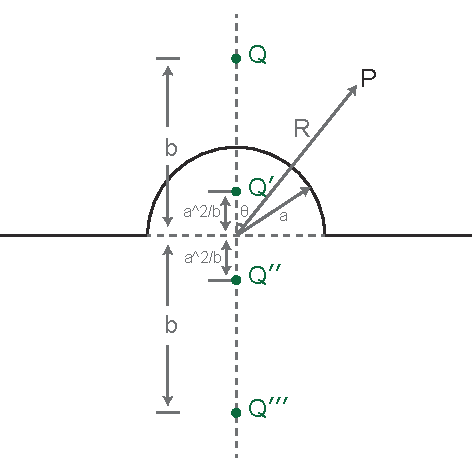
\includegraphics[width=10cm]{img/2.1/电像法1.pdf}
        \caption{导体平面上的半球}
        \label{2.1_fig:电像法1}
    \end{figure}
    
    如图\ref{2.1_fig:电像法1}放置三个镜像电荷\nota{Q'}、\nota{Q''}、\nota{Q'''}。它们的带电荷量分别为
    \begin{eqnarray}
        Q'   &=& -\frac{a}{b}Q \\
        Q''  &=& +\frac{a}{b}Q \\
        Q''' &=& -Q
    \end{eqnarray}
    这一的镜像电荷放置方案是由我们熟知的接地无穷大导体平面、接地导体球的镜像方案组合而成。容易看出,对于球面电势为0条件而言,\nota{Q}和\nota{Q'}作为一对镜像电荷使球面使球面等势为0,\nota{Q''}和\nota{Q'''}作为一对镜像电荷使球面等势为0,则它们的叠加当然也满足球面等势为0;对于导体平面电势为0条件而言,\nota{Q}和\nota{Q'''}作为一对镜像电荷使导体平面电势为0,\nota{Q'}和\nota{Q''}作为一对镜像电荷使导体平面电势为0,则它们的叠加当然也满足导体平面电势为0。
    
    这一以来,由静电场的唯一性定理可知,有如下唯一的电势解
    \begin{multline}
        \ph(R,\theta,\phi) = \frac{Q}{4\pi\eps_0 R}
        \left[
            \frac{+1}{\sqrt{1+\left(\frac{b}{R}\right)^2-2\left(\frac{b}{R}\right)\c}}
            +\frac{-1}{\sqrt{1+\left(\frac{b}{R}\right)^2+2\left(\frac{b}{R}\right)\c}}
            \right.
            \\
            \left.
            +\frac{-a/b}{\sqrt{1+\left(\frac{a^2}{bR}\right)^2-2\left(\frac{a^2}{bR}\right)\c}}
            +\frac{+a/b}{\sqrt{1+\left(\frac{a^2}{bR}\right)^2+2\left(\frac{a^2}{bR}\right)\c}}
        \right]
        \quad(R>a,0\le\theta<\pit)
    \end{multline}
    当然也容易验证,当\nota{R=a}或\nota{\theta=\pit}时,\nota{\ph(R,\theta,\phi)\equiv 0}。
    
    对于导体平面及其下方的区域,由于静电屏蔽,有
    \equa{
        \ph(R,\theta,\phi)\equiv 0 \quad(0\le R\le a\cup\pit\le\theta\le\pi)
    }

\question{有一点电荷\nota{Q}位于两个相互垂直的接地导体平面所围成的直角空间内,它到两个平面的距离为\nota{a}和\nota{b},求空间电势.}

    \begin{figure}[htbp]
        \centering
        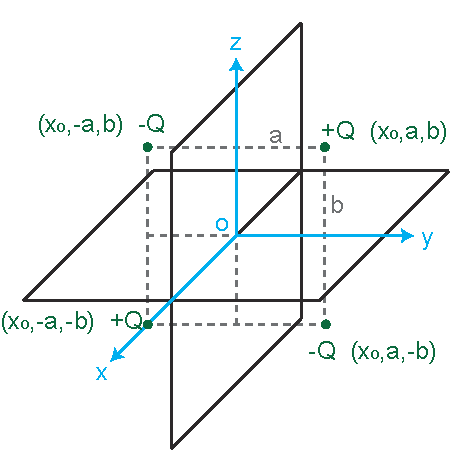
\includegraphics[width=10cm]{img/2.1/电像法2.pdf}
        \caption{两个垂直的导体平面}
        \label{2.1_fig:电像法2}
    \end{figure}
    
    如图\ref{2.1_fig:电像法2}放置三个镜像电荷,电荷量和坐标都已标示在图中。这一镜像电荷放置方案使根据单个无穷大接地 导体平面模型组合而来的,镜像电荷两两使得导体平面电势为零。
    
    由静电场的唯一性定理可知,有如下唯一的电势解
    \begin{multline}
        \ph(R,\theta,\phi)=\\
        \left\{
        \begin{aligned}
        	&\frac{Q}{4\pi\eps_0}
        	\left[ 
        	    \frac{+1}{\sqrt{(x-x_0)^2+(y-a)^2+(z-b)^2}}
        	    +\frac{-1}{\sqrt{(x-x_0)^2+(y+a)^2+(z-b)^2}}\right.&  \\
        	    &\left.+\frac{-1}{\sqrt{(x-x_0)^2+(y-a)^2+(z+b)^2}}
        	    +\frac{+1}{\sqrt{(x-x_0)^2+(y+a)^2+(z+b)^2}}
        	\right],
        	&(y>0,z>0)\\
        	& \qquad\qquad\qquad\qquad\qquad\qquad\qquad\qquad 0, &
        	\mathrm{else}
    	\end{aligned}
        \right.
    \end{multline}
    

\question{(附加题)一半径为\nota{R_0}的球面,在球坐标\nota{0<\theta<\frac{\pi}{2}}的半球面上电势为\nota{\ph_0},在\nota{\frac{\pi}{2}<\theta<\pi}的半球面上电势为\nota{-\ph_0},求空间各点电势.}

    \def \g{G(R,\theta,\phi;R',\theta',\phi')}
    \def \gr{Green函数}

    本题为第一类边值问题,定义Green函数为
    \equa{
        \nabla^2\g=-\frac{1}{\eps_0}\delta(R-R',\theta-\theta',\phi-\phi')
        \quad (0<R<R_0\cup R>R_0) \label{2.1_格林函数定义1}
    }
    \equa{
        \g|_{R=R_0}=0 \label{2.1_格林函数定义2}
    }
    原则上来讲,球内球外的\gr{}需要分别定义,因为它们是两个独立的求解区域。这里只是简便地将它们写成同一个格林函数,毕竟它们的解恰好在形式上是相同的,为
    \begin{multline}
        \g =\\ \frac{1}{4\pi\eps_0}
        \left[
            \frac{1}{\sqrt{R^2+R^2-2RR'\cos(\theta-\theta')}}
            -\frac{1}{\sqrt{\left(\frac{RR'}{R_0}\right)^2+R_0^2-2RR'\cos(\theta-\theta')}}
        \right]\label{2.1_格林函数的解}
    \end{multline}
    并且该解中的\nota{R,\theta,\phi}和\nota{R',\theta',\phi'}在形式上是对称的,因此可以将
    \equa{G(R',\theta',\phi';R,\theta,\phi)=\g=G}
    都简记为\nota{G}。
    
    在球内和球外无自由电荷,即
    \equa{\rho(R',\theta',\phi')=0} \label{2.1_自由电荷}
    根据Green formula得到电势解的形式
    \equa{
        \ph(R,\theta,\phi)=\eps_0\int\limits_{R'=R_0}\ph(R',\theta',\phi')
        \frac{\partial}{\partial n}G(R',\theta',\phi';R,\theta,\phi)\d S' \label{2.1_格林公式}
    }
    其中已代入(\ref{2.1_格林函数定义2})(\ref{2.1_自由电荷})来化简。
    
    球内和球外关于球面法向\nota{n}的定义是不同的,由此(\ref{2.1_格林公式})具体写为
    \begin{multline}
        \ph(R,\theta,\phi)=\\
        \left\{
        \begin{aligned}
        	&-2\pi\eps_0 R_0^2
        	\left[  
        	    \int_0^{\pit}\ph_0\left.\frac{\partial G}{\partial R'}\right|_{R'=R_0}\sin\theta\d\theta\right. & \\
        	    &\left.\qquad\qquad\qquad + \int_\pit^{\pi}\left(-\ph_0\right)\left.\frac{\partial G}{\partial R'}\right|_{R'=R_0}\sin\theta\d\theta
        	\right] 
        	&\left(R>R_0\right)& \\
        	&-2\pi\eps_0 R_0^2
        	\left[  
        	    \int_0^{\pit}\ph_0\left(-\left.\frac{\partial G}{\partial R'}\right|_{R'=R_0}\right)\sin\theta\d\theta\right. & \\
        	    &\left.\qquad\qquad\qquad + \int_\pit^{\pi}\left(-\ph_0\right)\left(-\left.\frac{\partial G}{\partial R'}\right|_{R'=R_0}\right)\sin\theta\d\theta
        	\right] 
        	&\left(0<R<R_0\right)& 
    	\end{aligned}
        \right.\label{2.1_电势解}
    \end{multline}
    其中
    \equa{
        \left.\frac{\partial G}{\partial R'}\right|_{R'=R_0}=\frac{1}{4\pi\eps_0 R_0^2}\frac{r^2-1}{\left[1+r^2-2r\cos(\theta-\theta')\right]^{\frac{3}{2}}}\label{2.1_8}
    }
    并已简记
    \equa{r=\frac{R}{R_0}>0}\label{2.1_9}
    % \equa{z_0=\cos\theta}\label{2.1_10}
    
    将(\ref{2.1_8})(\ref{2.1_9})代入(\ref{2.1_电势解})得
    \begin{equation}
        \ph(R,\theta,\phi)=
        \left\{
        \begin{aligned}
        	&-\frac{\ph_0}{2}
        	\left(\int_0^{\pit}-\int_{\pit}^{\pi}\right)
        	\frac{r^2-1}{\left[1+r^2-2r\cos(\theta-\theta')\right]^{\frac{3}{2}}}\sin\theta'\d\theta'
        	&r>1 \\
        	&\frac{\ph_0}{2}
        	\left(\int_0^{\pit}-\int_{\pit}^{\pi}\right)
        	\frac{r^2-1}{\left[1+r^2-2r\cos(\theta-\theta')\right]^{\frac{3}{2}}}\sin\theta'\d\theta'
        	&r<1
    	\end{aligned}
        \right.
    \end{equation}
    将源点最后的自由度\nota{\theta'}积掉,就可以(再不济也能在数值层面)得到电势\nota{\ph(R,\theta,\phi)}的表达式。该过程涉及第二类椭圆积分,我就不给出结果了。
    
    有趣的是,我们发现球内和球外的电势在形式上只相差一个负号。我们可以把它们统一写为
    \begin{equation}
        \ph(R,\theta,\phi)=
    	-\frac{\ph_0}{2}
    	\left(\int_0^{\pit}-\int_{\pit}^{\pi}\right)
    	\frac{\left|r^2-1\right|}{\left[1+r^2-2r\cos(\theta-\theta')\right]^{\frac{3}{2}}}\sin\theta'\d\theta'
    \end{equation}


% \chapter{静磁场}
%     \question{考虑载电流\nota{I}的无穷长细直导线,利用毕奥-萨伐尔定律,通过直接积分求磁感应强度。}

    \begin{figure}[htbp]
        \centering
        \includegraphics{img/3.1/导线.eps}
        \caption{无穷长直导线}
        \label{3.1_fig:导线}
    \end{figure}
    
    如图\ref{3.1_fig:导线},取导线沿\nota{z}轴,设\nota{P}点到导线的垂直距离为\nota{R},电流元\nota{I\d z}到\nota{P}点的矢径为\nota{\r},有毕奥-萨伐尔定律
    \begin{equation}
        B(P) = \frac{\mu I}{4\pi}\int_{-\infty}^{+\infty}
        \frac{\d \z\times \r}{r^3}\label{3.1_1}
    \end{equation}
    如图\ref{3.1_fig:导线},设\nota{\r}与\nota{\bm R}的夹角为\nota{\theta},注意到几何关系
    \begin{equation}
        |\d \z| = R \frac{1}{\cos^2\theta}\d \theta\label{3.1_2}
    \end{equation}
    \begin{equation}
        \d \z \times \r = |\d \z| r \cos \theta \danwei{\phi}\label{3.1_3}
    \end{equation}
    \begin{equation}
        r = \frac{R}{\cos\theta}\label{3.1_4}
    \end{equation}
    由(\ref{3.1_1})(\ref{3.1_2})(\ref{3.1_3})(\ref{3.1_4})得
    \begin{equation}
        B(P) = \frac{\mu I\danwei{\phi}}{4\pi R}\int_{-\pit}^{+\pit}\cos\theta\d \theta = \frac{\mu I\danwei{\phi}}{2\pi R}\label{3.1_5}
    \end{equation}

\question{求下面两个矢势对应的磁感应强度:}

    \subquestion{\nota{A_x = A_y = 0,\quad A_z = -y B_0}(其中\nota{\bz}为常数);}
    
    根据矢势的定义,可以直接写出
    \begin{equation}
        \b = \nabla \times \a = \dreieinss \ep \partial_i A_j \bm{e}_k = -\bz \bm{e}_x
    \end{equation}
    
    \subquestion{\nota{A_x = A_z = 0,\quad A_y = x B_0}(其中\nota{\bz}为常数)。}
    
    \begin{equation}
        \b = \nabla \times \a = \dreieinss \ep \partial_i A_j \bm{e}_k = \bz \bm{e}_z
    \end{equation}

%     \question{参考教材,}

    \subquestion{推导稳定超导电流满足的方程\equa{\nabla^2\j_s=\frac{1}{\lambda_L^2}\j_s}其中\nota{\lambda_L}是伦敦穿透深度。}
    
        伦敦第二方程
        \equa{\xuandu\j_s=-\alpha\b\label{3.2_1}}
        对(\ref{3.2_1})取旋度并利用恒定条件
        \equa{\sandu\j_s=0}
        以及麦克斯韦方程组
        \equa{\xuandu\b=\mu_0\j_s}
        进行化简
        \equa{\xuandu\kuohao{\xuandu\j_s}=-\alpha\kuohao{\xuandu\b}}
        \equa{\nabla\kuohao{\sandu\j_s}-\nabla^2\j_s=-\alpha\mu_0\j_s}
        \equa{\nabla^2\j_s=\frac{1}{\lambda_L^2}\j_s\label{3.2_2}}
        其中
        \equa{\lambda_L=\frac{1}{\sqrt{\mu_0\alpha}}}
        
    
    \subquestion{若超导体充满在\nota{z<0}的空间,并已知在\nota{z=0}处有稳定超导电流密度为\nota{\j_s(0)},方向沿\nota{x}方向,求超导体中的稳定超导电流密度。}
    
        由于系统具有x,y方向连续平移对称性
        \equa{\pd{^2}{x^2}=\pd{^2}{y^2}=0}
        则(\ref{3.2_2})转化为
        \equa{\frac{\d^2}{\d z^2}\j_s(z)=\frac{1}{\lambda_L^2}\j_s(z)\qquad(z<0)}
        其具有物理意义的解为
        \equa{\j_s(z)=\j_s(0)\mathrm{e}^{-z/\lambda_L}}
    
\question{半径为\nota{a}、处于理想迈斯纳态的超导球附近,距球心为\nota{d(d>a)}处有一沿球径方向的磁偶极子\nota{\m}。证明:\nota{\m}的镜像为\nota{\m'=-\kuohao{a/d}^3\m},位置在球内\nota{z={a^2}/{d}}处。}

    只需验证磁场解满足边界条件
    \equa{B_n=0\label{3.2_bianj}}
    由于不存在自由电流,可以引入磁标势来描述磁场,磁偶极子的磁标势解为
    \equa{\varphi_m^{(1)}=\frac{\m\cdot\bm{R}}{4\pi R^3}}
    \equa{\b^{(1)}=\nabla\varphi_m^{(1)}}
    其中
    \equa{\bm{R}=\bm{x}-\bm{x'}}
    
    如果\nota{\m}的镜像为\nota{\m'=-\kuohao{a/d}^3\m},位置在球内\nota{z={a^2}/{d}}处,则以磁偶极子所沿的球径方向取极轴,建立球坐标系,外部空间中的磁标势为
    \equa{
        \begin{aligned}
            \varphi_m
            &=
            \frac{m(r\cos\theta-d)}{\fkuohao{r^2+d^2-2rd\cos\theta}^{\frac{3}{2}}}-
            \frac{\kuohao{\frac{a}{d}}^3m\kuohao{r\cos\theta-\frac{a^2}{d}}}{\fkuohao{r^2+\kuohao{\frac{a^2}{d}}^2-2r\kuohao{\frac{a^2}{d}}\cos\theta}^{\frac{3}{2}}} \\
            &=
            \frac{m(r\cos\theta-d)}{\fkuohao{r^2+d^2-2rd\cos\theta}^{\frac{3}{2}}}-
            \frac{m\kuohao{r\cos\theta-\kuohao{\frac{a}{d}}^2d}}{\fkuohao{a^2+\kuohao{\frac{r}{a}}^2d^2-2rd\cos\theta}^{\frac{3}{2}}}
        \end{aligned}
    }
    则在边界上有
    \equa{
        \begin{aligned}
            B_n
            &=-\left.\pd{\varphi_m}{r}\right|_{r\to a}\\
            &=
            -\frac{m\cos\theta}{\fkuohao{a^2+d^2-2ad\cos\theta}^{\frac{3}{2}}}
            +\frac{3}{2}m\kuohao{a\cos\theta-d}\frac{2a-2d\cos\theta}{\fkuohao{a^2+d^2-2ad\cos\theta}^{\frac{5}{2}}}\\
            &\quad
            +\frac{m\cos\theta}{\fkuohao{a^2+d^2-2ad\cos\theta}^{\frac{3}{2}}}
            -\frac{3}{2}m\kuohao{a\cos\theta-\kuohao{\frac{a}{d}}^2d}\frac{2\kuohao{\frac{a}{d}}^2a-2d\cos\theta}{\fkuohao{a^2+d^2-2ad\cos\theta}^{\frac{5}{2}}}\\
            &=3m\frac{\kuohao{a\cos\theta-d}\kuohao{a-d\cos\theta}-\kuohao{\frac{a}{d}}\kuohao{a-d\cos\theta}\kuohao{\frac{d}{a}}\kuohao{a\cos\theta-d}}{\fkuohao{a^2+d^2-2ad\cos\theta}^{\frac{5}{2}}}\\
            &=0
        \end{aligned}
    }
    满足边界条件(\ref{3.2_bianj}),由唯一性定理可知,该镜像即唯一解。
    


% \chapter{电磁波的传播}
%     \question{考虑两列电场振幅振幅分别为\nota{E_1}和\nota{E_2}、偏振方向相同、初始相位同为零、频率分别为\nota{\omega+\d\omega}和\nota{\omega-\d\omega}的线偏振平面波,它们都沿\nota{z}轴转播。}

    \subquestion{求合成电磁波,并把合成电磁波写成以\nota{\omega}为频率的振幅被调制(即振幅依赖于空间坐标和时间)的平面波;}
    
    先简单地考虑真空(无色散)情形。两列波叠加后的电场为
    \equa{
        \begin{aligned}
            \e(z,t)
            &=\bm{e}_0 E_1\mathrm{e}^{\i\fkuohao{\kuohao{k+\d k}z-\kuohao{\o+\d\o}t}}
            +\bm{e}_0 E_2\mathrm{e}^{\i\fkuohao{\kuohao{k-\d k}z-\kuohao{\o-\d\o}t}}\\
            &=\bm{e}_0\mathrm{e}^{\i\kuohao{kz-\o t}}
            \fkuohao{ E_1\mathrm{e}^{\i\kuohao{z\d k-t\d\o}}+ E_2\mathrm{e}^{-\i\kuohao{z\d k-t\d\o}}}\\
            &=\bm{e}_0\mathrm{e}^{\i\kuohao{kz-\o t}}
            \fkuohao{\kuohao{ E_1+ E_2}\cos\kuohao{z\d k-t\d\o}+\kuohao{ E_1- E_2}\i\sin\kuohao{z\d k-t\d\o}}
        \end{aligned}
        \label{4.1_1}
    }
    其中记
    \equa{k=\o/c\qquad\d k=\d\o/c\label{4.1_2}}
    (\ref{4.1_1})中因子
    \equa{\widetilde{E}_0(z\d k-t\d\o)=\kuohao{ E_1+ E_2}\cos\kuohao{z\d k-t\d\o}+\kuohao{ E_1- E_2}\i\sin\kuohao{z\d k-t\d\o}}即为调制振幅。
    
    \subquestion{求合成波的相位传播速度和振幅波传播速度。}
    
    观察相位因子\nota{\mathrm{e}^{\i\kuohao{kz-\o t}}},显然其传播速度即相速度为
    \equa{v_p=\frac{\o}{k}=c\label{4.1_3}}
    而振幅波\nota{\widetilde{E}_0(z\d k-t\d\o)}的传播速度为
    \equa{v_g=\frac{\d\o}{\d k}=c\label{4.1_4}}
    
    在一般的介质中,通常有色散,则(\ref{4.1_2})改写为
    \equa{k=\o\sqrt{\mu(\o)\eps(\o)}}
    以及线性近似
    \equa{\d k = \kuohao{\sqrt{\mu(\o)\eps(\o)}+\o\pd{}{\o}\sqrt{\mu(\o)\eps(\o)}}\d\o}
    于是结果(\ref{4.1_3})(\ref{4.1_4})改为
    \equa{v_p=\frac{1}{\sqrt{\mu(\o)\eps(\o)}}}
    \equa{v_g=\frac{1}{\kuohao{\sqrt{\mu(\o)\eps(\o)}+\o\pd{}{\o}\sqrt{\mu(\o)\eps(\o)}}}\approx\frac{1}{\sqrt{\mu(\o)\eps(\o)}}\kuohao{1-\frac{\o}{\sqrt{\mu(\o)\eps(\o)}}\pd{\sqrt{\mu(\o)\eps(\o)}}{\o}}}
    
\question{从真空麦克斯韦方程组推导磁场满足的波动方程,以及磁场时谐波所满足的亥姆霍兹方程。}

    真空中的麦克斯韦方程组
    \equa{\xuandu\e=-\pd{\b}{t}\label{4.1_mx1}}
    \equa{\xuandu\b=\mu_0\eps_0\pd{\e}{t}\label{4.1_mx2}}
    \equa{\sandu\e=0\label{4.1_mx3}}
    \equa{\sandu\b=0\label{4.1_mx4}}
    对(\ref{4.1_mx2})两边取旋度,并结合(\ref{4.1_mx4})(\ref{4.1_mx1})化简
    \equa{\xuandu{\kuohao{\xuandu{\b}}}=\nabla\kuohao{\sandu\b}-\nabla^2\b=\mu_0\eps_0\pd{}{t}\kuohao{\xuandu\e}}
    \equa{\nabla^2\b-\frac{1}{c^2}\pd{^2}{t^2}\b=0\label{4.1_bod}}
    此即磁场满足的波动方程,其中
    \equa{c=\frac{1}{\sqrt{\mu_0\eps_0}}}
    
    考虑单模时谐解
    \equa{\b(x,t)=\b(x)\mathrm{e}^{-\i\o t}}
    则对(\ref{4.1_bod})替换
    \equa{\pd{}{t}\longrightarrow  -\i\o}
    得
    \equa{\nabla^2\b+k^2\b=0}
    此即磁场的亥姆霍兹方程,其中
    \equa{k=\frac{\o}{c}}


%     \question{考虑平面电磁波在两种线性各向同性介质的界面的反射和折射,设界面是无穷大光滑平面。根据麦克斯韦方程组和边值关系,分别对入射电场垂直入射面和平行入射面两种情形推导反射电场与入射电场的比、折射电场与入射电场的比,并给出反射率的表达式。请自行定义相关物理量的记号。}

    \begin{figure}[htbp]
        \centering
        \includegraphics[width=6cm]{img/4.2/正交系.png}
        \caption{正方向定义}
        \label{4.2_fig:正方向定义}
    \end{figure}

    设入射波的单模平面波解为
    \equa{\e_i=\e_{i0}\exp{\i\kuohao{\k_i\cdot\x-\o_it}}\label{4.2_pm1}}
    设反射波的单模平面波解为
    \equa{\e_r=\e_{r0}\exp{\i\kuohao{\k_r\cdot\x-\o_rt}}\label{4.2_pm2}}
    设折射波的单模平面波解为
    \equa{\e_t=\e_{t0}\exp{\i\kuohao{\k_t\cdot\x-\o_tt}}\label{4.2_pm3}}
    设界面为\nota{z=0}平面,\nota{z<0}为介质1,\nota{z>0}为介质2,电磁波从介质1射向介质2。设入射角为\nota{\theta_i},反射角为\nota{\theta_r},折射角为\nota{\theta_t}。对于电场p波(电场偏振方向平行于入射面)、电场s波(电场偏振方向垂直于入射面)、波矢\nota{\k}的正方向定义如图\ref{4.2_fig:正方向定义}所示。
    
    电场的边值关系
    \equa{\bm{e}_z\times\kuohao{\e_i+\e_r}=\bm{e}_z\times\e_t\label{4.2_bianze}}
    要对任意\nota{\x\in\{z=0\}}成立,则(根据线性无关性)必须有
    \equa{\o_i=\o_r=\o_t=\o\label{4.2_边值关系1}}
    \equa{\bm{e}_z\times\k_i=\bm{e}_z\times\k_r=\bm{e}_z\times\k_t\label{4.2_边值关系2}}
    即
    \equa{k_i\sin\theta_i=k_r\sin\theta_r=k_t\sin\theta_t\label{4.2_k1}}
    在介质中有
    \equa{k_i=k_r=\o\sqrt{\mu_1\eps_1}\label{4.2_k2}}
    \equa{k_t=\o\sqrt{\mu_2\eps_2}\label{4.2_k3}}
    由(\ref{4.2_k1})(\ref{4.2_k2})(\ref{4.2_k3})得
    \equa{\theta_i=\theta_r\label{4.2_反射定律}}
    \equa{\sqrt{\mu_1\eps_1}\sin\theta_i=\sqrt{\mu_2\eps_2}\sin\theta_t\label{4.2_折射定律}}
    此即反射定律和折射定律。
    
    再考虑磁场的边值关系
    \equa{\bm{e}_z\times\kuohao{\h_i+\h_r}=\bm{e}_z\times\h_t\label{4.2_bianzh}}
    以及电磁波中磁场和电场的关系
    \equa{\h=\sqrt{\frac{\eps}{\mu}}\bm{e}_k\times\e\label{4.2_he}}
    
    如果电场偏振方向垂直于入射面(即s波)   将单模平面波解(\ref{4.2_pm1})(\ref{4.2_pm2})(\ref{4.2_pm3})以及反射定律(\ref{4.2_反射定律})代入(\ref{4.2_bianze})(\ref{4.2_bianzh})(\ref{4.2_he})中(尤其注意正方向如图\ref{4.2_fig:正方向定义}不要弄错)得
    \equa{
        \begin{pmatrix}
            1 &
            -1 \\
            \sqrt{\eps_1/\mu_1}\cos\theta_i &
            \sqrt{\eps_2/\mu_2}\cos\theta_t
        \end{pmatrix}
        \begin{pmatrix}
            E_r \\ E_t
        \end{pmatrix}
        =
        \begin{pmatrix}
            -1 \\ \sqrt{\eps_1/\mu_1}\cos\theta_i
        \end{pmatrix}
        E_i
    }
    解得
    \equa{
        \frac{E_r}{E_i}=
        \frac{\epmua\cos\theta_i-\epmub\cos\theta_t}{\epmua\cos\theta_i+\epmub\cos\theta_t}\label{4.2_s反射}
    }
    \equa{
        \frac{E_t}{E_i}=
        \frac{2\epmua\cos\theta_i}{\epmua\cos\theta_i+\epmub\cos\theta_t}
    }
    
    振幅反射率即(\ref{4.2_s反射}),强度反射率/能流密度反射率则为
    \equa{R=\kuohao{\frac{E_r}{E_i}}^2=\kuohao{\frac{\epmua\cos\theta_i-\epmub\cos\theta_t}{\epmua\cos\theta_i+\epmub\cos\theta_t}}^2}
    不过,需要注意对于折射而言,强度折射率和能流密度折射率是不同的,这里就不展开了。
    
    如果电场偏振方向平行于入射面(即p波)   将单模平面波解(\ref{4.2_pm1})(\ref{4.2_pm2})(\ref{4.2_pm3})以及反射定律(\ref{4.2_反射定律})代入(\ref{4.2_bianze})(\ref{4.2_bianzh})(\ref{4.2_he})中(尤其注意正方向如图\ref{4.2_fig:正方向定义}不要弄错)得
    \equa{
        \begin{pmatrix}
            \cos\theta_i &
            \cos\theta_t \\
            \epmua &
            -\epmub
        \end{pmatrix}
        \begin{pmatrix}
            E_r \\ E_t
        \end{pmatrix}
        =
        \begin{pmatrix}
            \cos\theta_i \\ -\epmua
        \end{pmatrix}
        E_i
    }
    解得
    \equa{
        \frac{E_r}{E_i}=
        \frac{-\epmua\cos\theta_t+\epmub\cos\theta_i}{\epmua\cos\theta_t+\epmub\cos\theta_i}\label{4.2_p反射}
    }
    \equa{
        \frac{E_t}{E_i}=
        \frac{2\epmua\cos\theta_i}{\epmua\cos\theta_t+\epmub\cos\theta_i}
    }
    
    振幅反射率即(\ref{4.2_p反射}),强度反射率/能流密度反射率则为
    \equa{R=\kuohao{\frac{E_r}{E_i}}^2=\kuohao{\frac{-\epmua\cos\theta_t+\epmub\cos\theta_i}{\epmua\cos\theta_t+\epmub\cos\theta_i}}^2}

\question{考虑电场平行入射平面的平面电磁波从真空入射到无穷大光滑玻璃平面,设玻璃折射率为\nota{n=1.5}。\label{4.2_题2}}

    \subquestion{根据菲涅耳公式,画出反射电场与入射电场的比作为入射角函数的函数曲线;画出折射电场与入射电场的比作为入射角函数的函数曲线。}
    
    \begin{tcolorbox}[breakable, size=fbox, boxrule=1pt, pad at break*=1mm,colback=cellbackground, colframe=cellborder]
    \prompt{In}{incolor}{in}{\boxspacing}
        \begin{matcode}   
            % para
            n1 = 1;
            n2 = 1.5;
            
            % prec
            i  = linspace(0, pi/2, 100);
            si = sin(i);
            ci = cos(i);
            st = n1 / n2 * si;
            ct = sqrt( 1 - (n1/n2)^2 * si.^2 );
            
            % calc
            R  = ( -n1 * ct + n2 * ci ) ./ ( n1 * ct + n2 * ci );
            T  = ( 2 * n1 * ci ) ./ ( n1 * ct + n2 * ci );
            
            % plot
            figure;
            plot(i, R, "LineWidth", 3, "Color", 'r');
            hold on;
            plot(i, T, "LineWidth", 3, "Color", 'b');
            legend('反射', '折射')
            xlabel('入射角 (rad)');
            ylabel('振幅比');
            xticks([0, pi/8, pi/4, pi/8*3 , pi/2]);
            xticklabels({'0', '\pi/8', '\pi/4', '3\pi/4', '\pi/2'});
            ylim([-1, 1]);
            set(gca, 'FontSize', 16);
            set(gca, 'LineWidth', 1);
            grid on;
        \end{matcode}
    \end{tcolorbox}
    
    \begin{figure}[htbp]
    \prompt{Out}{outcolor}{out}{\boxspacing}
        \centering
        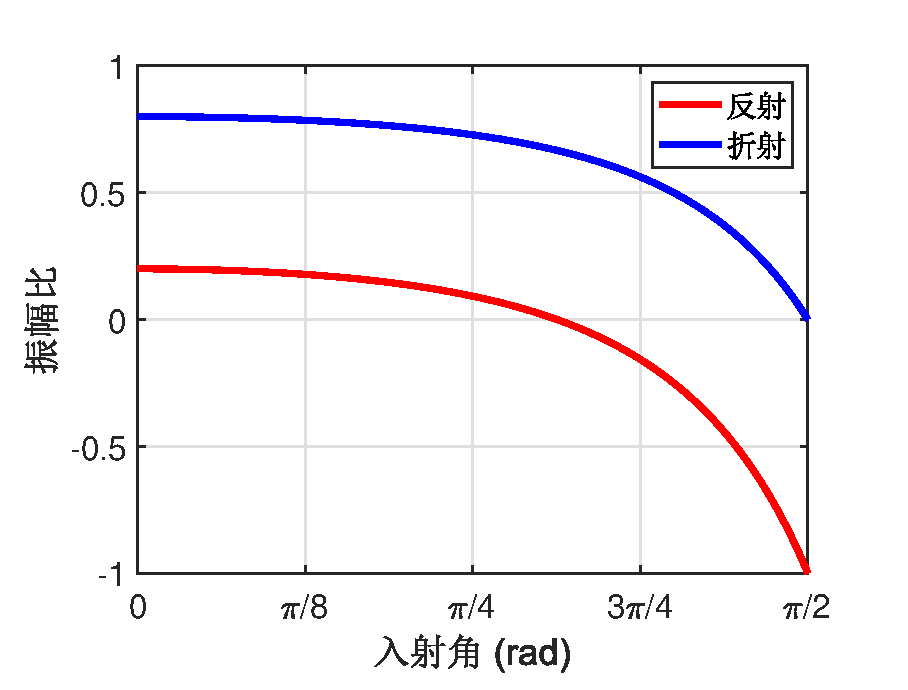
\includegraphics[width=10cm]{img/4.2/zwei.eps}
        \caption{振幅比随入射角的变化(从空气射入玻璃)}
        \label{4.2_fig:振幅比随入射角的变化(从空气射入玻璃)}
    \end{figure}
    
    \subquestion{求出布儒斯特角的数值。}
    
    可以用数值方法,从图\ref{4.2_fig:振幅比随入射角的变化(从空气射入玻璃)}中直接读出p波振幅反射比为0的入射角即布儒斯特角
    \equa{\theta_B=0.9828~\mathrm{rad}}
    
    也可以用解析的办法,令(\ref{4.2_p反射})取零,并考虑\nota{\mu_1\approx\mu_2}得
    \equa{\theta_i+\theta_t=\frac{\pi}{2}\label{4.2_tmp1}}
    又将折射定律(\ref{4.2_折射定律})改写为
    \equa{\sin\theta_i=n\sin\theta_t\label{4.2_tmp2}}
    由(\ref{4.2_tmp1})(\ref{4.2_tmp2})得
    \equa{\theta_B=\arctan n=0.9828~\mathrm{rad}}
    
\question{接上题,考虑平面光波从玻璃介质入射到玻璃和真空的无穷大光滑平面界面。求全反射角的数值。}

    可以用与题\ref{4.2_题2}类似的数值办法,找到强度反射比为1的入射角(这里以p波为例)
    
    \begin{tcolorbox}[breakable, size=fbox, boxrule=1pt, pad at break*=1mm,colback=cellbackground, colframe=cellborder]
    \prompt{In}{incolor}{in}{\boxspacing}
        \begin{matcode}   
            % para
            n1 = 1.5;
            n2 = 1;
            
            % prec
            i  = linspace(0, pi/2, 100);
            si = sin(i);
            ci = cos(i);
            st = n1 / n2 * si;
            ct = sqrt( 1 - (n1/n2)^2 * si.^2 );
            
            % calc
            R  = ( -n1 * ct + n2 * ci ) ./ ( n1 * ct + n2 * ci );
            T  = ( 2 * n1 * ci ) ./ ( n1 * ct + n2 * ci );
            R  = abs(R).^2;
            T  = abs(T).^2;
            
            % plot
            figure;
            plot(i, R, "LineWidth", 3, "Color", 'r');
            xlabel('入射角 (rad)');
            ylabel('p波强度反射率');
            xticks([0, pi/8, pi/4, pi/8*3 , pi/2]);
            xticklabels({'0', '\pi/8', '\pi/4', '3\pi/4', '\pi/2'});
            ylim([0, 1]);
            set(gca, 'FontSize', 16);
            set(gca, 'LineWidth', 1);
        \end{matcode}
    \end{tcolorbox}
    
    \begin{figure}[htbp]
    \prompt{Out}{outcolor}{out}{\boxspacing}
        \centering
        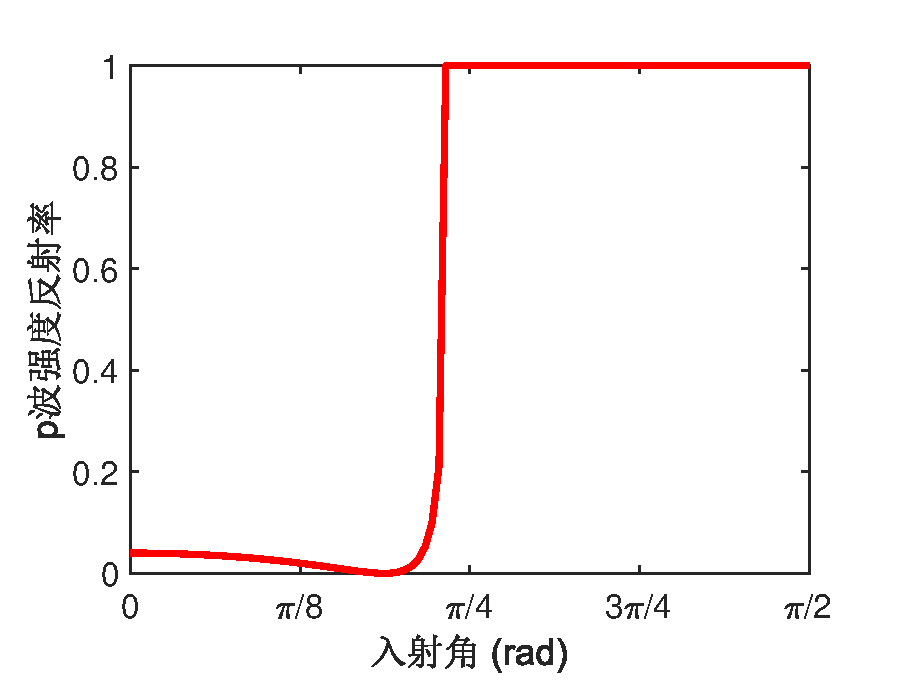
\includegraphics[width=10cm]{img/4.2/drei.eps}
        \caption{p波强度反射比随入射角的变化(从玻璃射入空气)}
        \label{4.2_fig:强度比随入射角的变化(从玻璃射入空气)}
    \end{figure}
    
    不过,需要注意的是这里考虑的应当是强度而非振幅,因为全反射会发生相移,使振幅反射/折射比为复数,直接画个实部是有失偏颇的。
    
    由此读出,全反射角
    \equa{\theta_c=0.7297~\mathrm{rad}}
    
    或者利用解析的办法也可容易地得出
    \equa{\theta_c=\arcsin\frac{1}{n}=0.7297~\mathrm{rad}}
    
\question{平面电磁波垂直射到金属表面上,试证明透入金属内部的电磁波能量全部变成焦耳热。}

    设金属界面为\nota{z=0}平面,\nota{z>0}为金属。设导体中波矢为
    \equa{\k=\bt+\i\ap=(\beta+\i\alpha)\bm{e}_z=k\bm{e}_z}
    金属中电场平面波
    \equa{\e=\e_0\exp{\i\kuohao{kz-\o t}}\label{4.2_4.1}}
    磁场波可由电场计算
    \equa{\h=\frac{1}{\o\mu}\k\times\e\label{4.2_4.2}}
    
    由(\ref{4.2_4.1})(\ref{4.2_4.2})计算进入金属界面的平均能流密度
    \equa{\langle\bm{S}\rangle = \frac{1}{2}\mathrm{Re}\kuohao{\e^*\times\h}=\frac{\beta}{2\o\mu}E_0^2\bm{e}_z\label{4.2_res1}}
    
    而根据欧姆定律
    \equa{\j=\sigma\e}
    则单位面积对应的焦耳热功率为
    \equa{\langle P\rangle=\int_0^\infty\frac{1}{2}\mathrm{Re}\kuohao{\j^*\times\e}\d z=\frac{\sigma E_0^2}{4\alpha}\label{4.2_res2}}
    由于垂直入射,有
    \equa{\alpha\beta=\frac{1}{2}\o\mu\sigma\label{4.2_res3}}
    由(\ref{4.2_res1})(\ref{4.2_res2})(\ref{4.2_res3})知
    \equa{\langle S\rangle=\langle P\rangle}
    
\question{平面电磁波由真空倾斜入射到导电介质表面上,入射角为\nota{\theta_1}。求导电介质中电磁波的相速度和衰减长度。若导电介质为金属,结果如何?}
    
    设平面单模波解如(\ref{4.2_pm1})(\ref{4.2_pm2})(\ref{4.2_pm3}),得其边值关系
    (\ref{4.2_边值关系1})(\ref{4.2_边值关系2})。这里只需要把折射波波矢\nota{\k_t}改写为复矢量
    \equa{\k_t=\bt+\i\ap\label{4.2_fu}}
    取xz平面为入射平面,记\nota{\theta_1=\theta_i}。由(\ref{4.2_边值关系2})(\ref{4.2_fu})得
    \equa{\alpha_x=\alpha_y=\beta_y=0\label{4.2_5.3}}
    \equa{\beta_x=k_i\sin\theta_i=\frac{\o}{c}\sin\theta_1\label{4.2_5.4}}
    
    导电介质中有亥姆霍兹方程
    \equa{\nabla^2\e_t+\o^2\mu\kuohao{\eps+\i\frac{\sigma}{\o}}\e_t=0\label{4.2_haim}}
    将(\ref{4.2_pm3})(\ref{4.2_fu})代入(\ref{4.2_haim})得
    \equa{\beta^2-\alpha^2=\o^2\mu\eps\label{4.2_5.1}}
    \equa{\ap\bt=\frac{1}{2}\o\mu\sigma\label{4.2_5.2}}
    
    由(\ref{4.2_5.3})(\ref{4.2_5.4})(\ref{4.2_5.1})(\ref{4.2_5.2})得
    \equa{\kuohao{\frac{\o}{c}\sin\theta_1}^2+\beta_z^2-\alpha_z^2=\o^2\mu\eps}
    \equa{\alpha_z\beta_z=\frac{1}{2}\o\mu\sigma}
    解得
    \equa{\beta_z^2=\frac{1}{2}\kuohao{\mu\eps\o^2-\frac{\o^2}{c^2}\sin^2\theta_1}+\frac{1}{2}\fkuohao{\kuohao{\mu\eps\o^2-\frac{\o^2}{c^2}\sin^2\theta_1}^2+\kuohao{\mu\sigma\o}^2}^\frac{1}{2}}
    \equa{\alpha_z^2=-\frac{1}{2}\kuohao{\mu\eps\o^2-\frac{\o^2}{c^2}\sin^2\theta_1}+\frac{1}{2}\fkuohao{\kuohao{\mu\eps\o^2-\frac{\o^2}{c^2}\sin^2\theta_1}^2+\kuohao{\mu\sigma\o}^2}^\frac{1}{2}}
    则相速度为
    \equa{v=\frac{\o}{\beta}=\frac{\o}{\sqrt{\beta_x^2+\beta_z^2}}}
    穿透深度为
    \equa{\delta=\frac{1}{\alpha}=\frac{1}{\sqrt{\alpha_z^2}}}
    
    若导电介质为金属,则有良导体条件
    \equa{\frac{\sigma}{\o\eps}\gg 1}
    从而
    \equa{k_t^2=\i\o\mu\sigma\kuohao{1-\i\frac{\o\eps}{\sigma}}\approx\i\o\mu\sigma}
    于是
    \equa{\beta^2-\alpha^2\approx0}
    \equa{\alpha_z\beta_z=\frac{1}{2}\o\mu\sigma=\frac{1}{2}\o^2\mu_0\eps_0\frac{\sigma}{\o\eps_0}\gg\frac{1}{2}\kuohao{\frac{\o}{c}}^2}
    即
    \equa{\alpha_z\beta_z\gg\beta_x^2}
    故得近似解
    \equa{\alpha\approx\beta\approx\sqrt{\frac{\o\mu\sigma}{2}}}
    则相速度为
    \equa{v=\frac{\o}{\beta}=\sqrt{\frac{2\o}{\mu\sigma}}}
    穿透深度为
    \equa{\delta=\frac{1}{\alpha}=\sqrt{\frac{2}{\o\mu\sigma}}}

%     \question{考虑矩形谐振腔如图,其中L3>L2>L1. 求\nota{f_{110}}模的磁强。考虑有效电导率,求单位表面的平均损耗功率。}

    \begin{figure}[htbp]
        \centering
        \includegraphics[width=8cm]{img/4.3/1.png}
        \caption{矩形谐振腔}
        \label{4.3_fig:矩形谐振腔}
    \end{figure}
    
    矩形谐振腔中的\nota{f_{110}}模驻波解为
    \equa{\e=E_0\exp{\i\o t}\sin\frac{\pi x}{L_1}\sin\frac{\pi y}{L_2}\bm{e}_z\label{4.3_1}}
    由时谐波的性质得到磁场
    \equa{
        \h=\frac{\exp{\i\o t}}{\i\o\mu}\xuandu\e
        =\frac{\pi E_0\exp{\i\o t}}{\i\o\mu}\kuohao{\frac{1}{L_2}\sin\frac{\pi x}{L_1}\cos\frac{\pi y}{L_2}\bm{e}_x-\frac{1}{L_1}\cos\frac{\pi x}{L_1}\sin\frac{\pi y}{L_2}\bm{e}_y}\label{4.3_2}
    }
    
    由于谐振腔内的驻波解是由理想导体的边界条件得到的,电磁波在导体界面全反射,显然由(\ref{4.3_1})(\ref{4.3_2})可直接算得边界上的平均能流密度为
    \equa{\langle\bm{S}\rangle = \frac{1}{2}\mathrm{Re}\kuohao{\e^*\times\h}=0}
    由于能量守恒,即理想导体边界无损耗功率。
    
    对于非理想导体,考虑良导体条件
    \equa{\xl\ll1}
    我们估计耗散功率密度\nota{p}的一阶小量,即
    \equa{p\sim\O{\xl}\sigma E_0^2}
    对于每个边界,我们从导体内深度为\nota{\xi}处的电流密度入手,计算耗散功率密度,并记\nota{\bm{e}_\xi}为从谐振腔指向导体内部的边界单位法向量。
    
    边界处的切向自由电流线密度矢量\nota{\af}可以由磁场的边界条件确定
    \equa{\af=-\bm{e}_\xi\times\h\label{4.3_af}}
    这里忽略了导体内的磁场,因为它远远小于谐振腔内的磁场\nota{\h}。根据郭硕鸿《电动力学》第四章\nota{\S3}的例2给出的结果,切向\nota{\af}引起的耗散功率体密度\nota{p_t}为
    \equa{p_t\sim\frac{\o\mu}{2}\af^*\cdot\af\exp{-2\alpha\xi}}
    其中
    \equa{\alpha=\sqrt{\frac{\o\mu\sigma}{2}}}
    我们先进行数量级的估算,由(\ref{4.3_2})(\ref{4.3_af})有
    \equa{\af^*\cdot\af\sim\frac{E_0^2}{\o^2\mu^2L^2}}
    于是
    \equa{p_t
        \sim\kuohao{\xl}\sigma\e_0^2\frac{1}{\mu\eps\o^2L^2}
        \sim\kuohao{\xl}\sigma\e_0^2\frac{c^2}{\o^2\lambda^2}\sim\O{\xl}\sigma\e_0^2}
    可见\nota{p_t}为我们要求的一阶小量。
    
    下面估算边界处导体内的法向电流密度的数量级。边界处自由电荷面密度\nota{\sigma_f}满足
    \equa{\sigma_f=-\eps\e\cdot\bm{e}_\xi}
    该式由高斯定律给出,且同样在计算中忽略导体腔内的电场,因为它远远小于谐振腔内电场\nota{\e}(需要注意的是,在计算耗散功率密度时不能忽略导体内电场,因为那个式子两边都是一阶小量)。由电荷的连续性方程可以估算法向电流密度的数量级
    \equa{J_\xi\kuohao{\xi,t}\sim-\pd{\sigma_f}{t}\sim\eps\o E_0}
    则这部分电流的耗散功率密度为
    \equa{p_n=\frac{J_\xi^2}{2\sigma}\sim\O{\kuohao{\xl}^2}\sigma E_0^2} 
    为二阶小量,远远小于切向电流引起的耗散功率密度\nota{p_t}。
    
    于是我们在计算中只需要考虑\nota{p_t}。由(\ref{4.3_2})(\ref{4.3_af})得各个面的耗散功率面密度为
    \equa{
        P_L=
        \left\{
        \begin{aligned}
            &\qquad\qquad\qquad\quad\frac{\pi^2\alpha}{2\sigma\o^2\mu^2}E_0^2\frac{1}{L^2_1}\sin^2\frac{\pi y}{L^2_2} & x=0,L_1 \\
            &\qquad\qquad\qquad\quad\frac{\pi^2\alpha}{2\sigma\o^2\mu^2}E_0^2\frac{1}{L^2_2}\sin^2\frac{\pi x}{L^2_1} & y=0,L_2 \\
            &\frac{\pi^2\alpha}{2\sigma\o^2\mu^2}E_0^2
            \kuohao{
                \frac{1}{L^2_1}\cos^2\frac{\pi x}{L^2_1}\sin^2\frac{\pi y}{L^2_2}+
                \frac{1}{L^2_2}\sin^2\frac{\pi x}{L^2_1}\cos^2\frac{\pi y}{L^2_2}
            }
            & z=0,L_3 \\
        \end{aligned}
        \right.
    }
    % \equa{
    %     P_L=
    %     \begin{cases}
    %         \frac{\pi^2\alpha}{2\sigma\o^2\mu^2}E_0^2\frac{1}{L^2_1}\sin^2\frac{\pi y}{L^2} & x=0,L_1 \\
    %         \frac{\pi^2\alpha}{2\sigma\o^2\mu^2}E_0^2\frac{1}{L^2_1}\sin^2\frac{\pi y}{L^2} & x=0,L_1 \\
    %         \frac{\pi^2\alpha}{2\sigma\o^2\mu^2}E_0^2\frac{1}{L^2_1}\sin^2\frac{\pi y}{L^2} & x=0,L_1 \\
    %     \end{cases}
    % }
    
    % 我们同样可以按照下面的方法考虑有限电导率,再取极限得到这一结果。考虑有限电导率为\nota{\sigma},且有良导体近似\nota{\bm{\alpha}\approx\bm{\beta}\approx(1/\delta)\e'_z},其中定义\nota{\e'_z}为谐振腔指向导体边界方向的法向量,穿透距离为\nota{z'}。在\nota{x=0,L_1}或\nota{y=0,L_2}的边界\nota{\e=0}故亦无电流穿透入导体,而在\nota{z=0,L_3}的边界则有有限的穿透深度。
    % \equa{\e'=E_0\exp{\i\o t}\sin\frac{\pi x}{L_1}\sin\frac{\pi x}{L_2}\exp{\i\kuohao{\beta+\i\alpha}z'}\e'_z}
    % \equa{\bm{J}=\sigma\e'}
    % 单位表面的平均耗散功率为
    % \equa{
    %     \langle P\rangle
    %     =\int_0^\infty\frac{1}{2}\mathrm{Re}\kuohao{\bm{J}^*\times\e'}\d z'
    %     =\frac{\sigma\delta}{4}\kuohao{E_0\sin\frac{\pi x}{L_1}\sin\frac{\pi x}{L_2}}^2
    % }
    % 针对\nota{f_{110}}模进一步化简得到
    % \equa{\langle P\rangle=\frac{1}{4}\sqrt{\frac{2\sigma}{\pi}}\fkuohao{\kuohao{\frac{1}{L_1^2}+\frac{1}{L_2^2}}\frac{\mu}{\eps}}^{-\frac{1}{2}}\kuohao{E_0\sin\frac{\pi x}{L_1}\sin\frac{\pi x}{L_2}}^2}
    % 有趣的是,这一结果显示,电导率\nota{\sigma}趋于无穷时,若不考虑超导效应,耗散功率居然是发散的。
    
\question{论证矩形波导管内不存在\nota{\mathrm{TM}_{m0}}或\nota{\mathrm{TM}_{0n}}波。}

    矩形波导管中的电场单模行波解为
    \begin{equation}
        \left\{
            \begin{aligned}
                    E_x&=A_1\cos(k_xx)\sin(k_yy)\exp{\i k_zz}\\
                    E_y&=A_2\sin(k_xx)\cos(k_yy)\exp{\i k_zz}\\
                    E_z&=A_3\sin(k_xx)\sin(k_yy)\exp{\i k_zz}\\
            \end{aligned}
        \right.
    \end{equation}
    \equa{k_x=\frac{m\pi}{a},\qquad k_y=\frac{n \pi}{b}\qquad(m,n=0,1,2,\cdots)\label{4.3_k}}
    由麦克斯韦方程
    \equa{\h=\frac{1}{\i\o\mu}\xuandu\e}
    得磁场解为
    \begin{equation}
        \left\{
            \begin{aligned}
                    H_x&=(k_yA_3-\i k_zA_2)\sin(k_xx)\cos(k_yy)\exp{\i k_zz}\\
                    H_y&=(\i k_zA_1-k_xA_3)\sin(k_xx)\cos(k_yy)\exp{\i k_zz}\\
                    H_z&=(k_xA_2-k_yA_1)\sin(k_xx)\cos(k_yy)\exp{\i k_zz}\\
            \end{aligned}
        \right.
    \end{equation}
    
    而\nota{\mathrm{TM}}波满足
    \equa{H_z=0}
    对于任意\nota{x,y,z}成立,即
    \nota{k_xA_2-k_yA_1=0\label{4.3_TM}}
    
    则\nota{\mathrm{TM}_{m0}}波要求
    \equa{n=0\label{4.3_n}}
    由(\ref{4.3_k})(\ref{4.3_TM})(\ref{4.3_n})得
    \equa{k_x=k_y=k_z=0}
    即
    \equa{\h_{\mathrm{TM}_{m0}}=0\qquad\e_{\mathrm{TM}_{m0}}=0}
    故矩形波导管内不存在\nota{\mathrm{TM}_{m0}}波。
    
    \nota{\mathrm{TM}_{0n}}波则要求
    \equa{m=0\label{4.3_m}}
    由(\ref{4.3_k})(\ref{4.3_TM})(\ref{4.3_m})得
    \equa{k_x=k_y=k_z=0}
    即
    \equa{\h_{\mathrm{TM}_{0n}}=0\qquad\e_{\mathrm{TM}_{0n}}=0}
    故矩形波导管内不存在\nota{\mathrm{TM}_{0n}}波。

%     \question{验证一维非线性薛定谔方程的亮孤子解。}

    一维非线性薛定谔方程
    \equa{\i\pd{ U}{\xi}=\kuohao{-\viervierban\ppd{}{s}+\be-\be\det{ U}\genh} U\label{4.4_非线性薛定谔方程}}
    要验证的孤子解
    \equa{ U=r\genh\sech\fkuohao{\kuohao{\be r}\genh s}\exp{\i\be\kuohao{\frac{r}{2}-1\xi}}\label{4.4_孤子解}}
    
    将(\ref{4.4_孤子解})代入(\ref{4.4_非线性薛定谔方程})右边第一项
    \equa{
        \begin{aligned}
            -\viervierban\ppd{}{s} U
            &= -\viervierban\kuohao{\be r}\genh \pd{}{s}\hkuohao{-\tanh\viervierx U} \\
            &= -\viervierban\be r\hkuohao{\tanh^2\viervierx U-\kuohao{1-\tanh^2\viervierx} U} \\
            &= -\be r\hkuohao{\tanh^2\viervierx-\viervierban} U
        \end{aligned}
        \label{4.4_第一项}
    }
    将(\ref{4.4_孤子解})代入(\ref{4.4_非线性薛定谔方程})右边第三项
    \equa{
        \begin{aligned}
            -\be\det{ U} U
            &= -\be r\sech^2\viervierx U \\
            &= -\be r\hkuohao{1-\tanh^2\viervierx} U
        \end{aligned}
        \label{4.4_第三项}
    }
    则由(\ref{4.4_第一项})(\ref{4.4_第三项})(\ref{4.4_孤子解})得(\ref{4.4_非线性薛定谔方程})右边为
    \equa{
        \begin{aligned}
            \mathrm{RHS.}
            &= -\viervierban\ppd{}{s} U-\be\det{ U}\genh U+\be U \\
            &= -\be r\hkuohao{\tanh^2\viervierx-\viervierban} U -\be r\hkuohao{1-\tanh^2\viervierx} U +\be U \\
            &= -\viervierban\be r+\be U 
        \end{aligned}
        \label{4.4_右边}
    }
    而将(\ref{4.4_孤子解})代入(\ref{4.4_非线性薛定谔方程})左边得
    \equa{
        \mathrm{LHS.}=-\be\kuohao{\frac{r}{2}-1} U =-\viervierban\be r+\be U
        \label{4.4_左边}
    }
    由(\ref{4.4_右边})(\ref{4.4_左边})可见
    \equa{\mathrm{RHS.}=\mathrm{LHS.}}
    则证明了(\ref{4.4_孤子解})为(\ref{4.4_非线性薛定谔方程})的解。


% \chapter{电磁波的辐射}
%     \question{写出电磁场强和电磁势的关系、一般规范变换。}

    电磁场强和电磁势的关系
    \equa{\b=\xuandu\a\label{5.1_矢势定义}}
    \equa{\e=-\tidu\ph-\pd{\a}{t}\label{5.1_标势定义}}
    
    一般规范变换
    \equa{\a\to\a'=\a+\tidu\psi}
    \equa{\ph\to\ph'=\ph-\pd{\psi}{t}}

\question{从真空麦克斯韦方程组推导一般电磁势满足的基本方程。}

    真空麦克斯韦方程组
    \equa{\xuandu\e=-\pd{\b}{t}\label{5.1_maxwell1}}
    \equa{\xuandu\h=\pd{\d}{t}+\j\label{5.1_maxwell2}}
    \equa{\sandu\d=\rho\label{5.1_maxwell3}}
    \equa{\sandu\b=0\label{5.1_maxwell4}}
    其中
    \equa{\d=\varepsilon_0\e\qquad\b=\muz\h}
    
    麦克斯韦方程组的\neq{5.1_maxwell1}和\neq{5.1_maxwell4}已经体现在电磁势的定义\neq{5.1_矢势定义}\neq{5.1_标势定义}中。对于剩下的\neq{5.1_maxwell2}\neq{5.1_maxwell3}两条,将\neq{5.1_矢势定义}\neq{5.1_标势定义}代入\neq{5.1_maxwell2}得
    \equa{\xuandu\kuohao{\xuandu\a}=\muz\varepsilon_0\pd{}{t}\kuohao{-\tidu\ph-\pd{\a}{t}}+\muz\j}
    即
    \equa{\tidu\kuohao{\sandu\a}-\tidu^2\a=-\frac{1}{c^2}\tidu\kuohao{\pd{\ph}{t}}-\frac{1}{c^2}\ppd{\a}{t}+\muz\j}
    其中
    \equa{\frac{1}{c^2}=\muz\varepsilon_0}
    移项、整理得
    \equa{\tidu^2\a-\frac{1}{c^2}\ppd{\a}{t}-\tidu\kuohao{\sandu\a+\frac{1}{c^2}\pd{\ph}{t}}=-\muz\j\label{5.1_达朗贝尔1}}
    又将\neq{5.1_矢势定义}\neq{5.1_标势定义}代入\neq{5.1_maxwell3}得
    \equa{\varepsilon_0\sandu\kuohao{-\tidu\ph-\pd{\a}{t}}=\rho}
    即
    \equa{\nabla^2\ph+\pd{}{t}\kuohao{\sandu\a}=\frac{\rho}{\varepsilon_0}\label{5.1_达朗贝尔2}}
    \neq{5.1_达朗贝尔1}\neq{5.1_达朗贝尔2}即为一般电磁势在真空中满足的基本方程。若取洛伦兹规范,则\neq{5.1_达朗贝尔1}\neq{5.1_达朗贝尔2}转化为达朗贝尔方程。

\question{证明\nota{f\kuohao{t-r/c}}满足下一维波动方程:\nota{\ppd{f}{r}-\frac{1}{c^2}\ppd{f}{t}=0}。}

    将\nota{f\kuohao{t-r/c}}的形式代入波动方程\nota{\ppd{f}{r}-\frac{1}{c^2}\ppd{f}{t}=0},得
    \equa{\mathrm{LHS.}=\ppd{}{r}f\kuohao{t-r/c}-\frac{1}{c^2}\ppd{}{t}f\kuohao{t-r/c}=\kuohao{-\frac{1}{c}}^2f''-\frac{1}{c^2}f''=0=\mathrm{RHS.}}
    证毕。

%     \question{计算圆形小孔的衍射。}

    考虑平面波入射,小孔半径为\nota{a},计算远场的夫琅禾费衍射\footnote{郭硕鸿《电动力学(第三版)》179页这个公式写错了,它的分子漏了一个\nota{k},量纲都不对呢。好多同学直接照抄课本,于是也写错了,这不好。}
    \equa{
        \begin{aligned}
            \psi\kuohao{\x}
            &= -\frac{\i k\psi_0\exp{\i kR}}{4\pi R}\kuohao{1+\cos\theta_2}\int_{S_0}\exp{-\i\k_2\cdot\x'}\d S' \\
            &= -\frac{\i k\psi_0\exp{\i kR}}{4\pi R}\kuohao{1+\cos\theta_2}\int_0^{2\pi}\int_0^a\exp{-\i k\sin\theta_2 R'\cos\phi}R'\d R' \d \phi \\
            &= -\frac{\i ka^2\psi_0\exp{\i kR}}{2 R} \kuohao{\frac{1+\cos\theta_2}{2}}
            \fkuohao{\frac{2J_1\kuohao{k_2a\sin\theta_2}}{k_2a\sin\theta_2}} \\
        \end{aligned}
    }
    其中\nota{J_1(x)}表示一阶Bessel函数。
    
    于是光强分布为
    \equa{I=\psi^*\psi=I_0\kuohao{\frac{1+\cos\theta_2}{2}}^2\fkuohao{\frac{2J_1\kuohao{k_2a\sin\theta_2}}{k_2a\sin\theta_2}}^2\label{5.2_I}}
    其中
    \equa{I_0=\kuohao{\frac{ka^2\psi_0}{2R}}^2}
    此即衍射图样中心的光强。
    
    在远场近轴条件下,往往只计算到\nota{\theta_2}的最低次项,于是\neq{5.2_I}近似为
    \equa{I\approx I_0\fkuohao{\frac{2J_1\kuohao{k_2a\theta_2}}{k_2a\theta_2}}^2}
    
    
\newpage
\question{设有一电矩振幅为\nota{\p},频率为\nota{\o}的电偶极子距理想导体平面为\nota{a/2}处,\nota{\p}平行于导体平面。设\nota{a\ll\lambda},求在\nota{R\gg\lambda}处电磁场及辐射能流。}

    对于电偶极子
    \equa{\p\kuohao{t}=\p_0\exp{\i\o t}}
    其产生的矢势场为(下面的场都是时谐场,简便起见,只写空间部分)
    \equa{\a\kuohao{\x}\exp{\i\o t}=\frac{\muz}{4\pi}\frac{\exp{\i kR}}{R}\dot{\p}=\frac{\muz}{4\pi}\frac{\exp{\i kR}}{R}\i\o\p_0\exp{\i\o t}}
    
    对于有镜像存在的情形,我们在远场条件近似到\nota{1/R}的最低次项,则总的矢势为
    \equa{\a_{\mathrm{tot}}=\bm{a}\cdot\tidu'\a=-\bm{a}\cdot\danwei{R}\i k\a=a\cos\theta\o k\frac{\muz}{4\pi}\frac{\exp{\i kR}}{R}\p_0}
    其中\nota{\bm{a}=a\danwei{n}}垂直于导体平面,从镜像偶极子指向真实偶极子。
    
    则可由此计算电磁场
    \equa{\b=\xuandu\a_{\mathrm{tot}}=\i ak^3c\cos\theta\frac{\muz}{4\pi}\frac{\exp{\i kR}}{R}\danwei{R}\times\p_0}
    \equa{\e=\frac{\i c}{k}\xuandu\b=\i ak^3c^2\cos\theta\frac{\muz}{4\pi}\frac{\exp{\i kR}}{R}\kuohao{\p_0-p_0\sin\theta\danwei{R}}}
    能流密度对时间的平均值为
    \equa{\langle\s\rangle=\frac{1}{2}\mathrm{Re}\kuohao{\e^*\times\h}=\frac{c}{2\mu}\det{\b}^2\danwei{R}=\frac{\muz\o^6a^2\cos^2\theta}{32\pi^2c^3R^2}\det{\danwei{R}\times\p_0}^2\danwei{R}}
    可以在球极坐标中表示,取北极轴沿\nota{\bm{a}},赤道面上的极轴沿\nota{\p_0},则
    \equa{\langle\s\rangle=\frac{\muz\o^6a^2p_0^2\cos^2\theta}{32\pi^2c^3R^2}\kuohao{\sin^2\phi+\cos^2\theta\cos^2\phi}}

\newpage
\question{设有线偏振平面波\nota{\e=\e_0\exp{\i\kuohao{kx-\o t}}}照射到一个绝缘介质球上(\nota{\e_0}在\nota{z}方向),引起介质球极化,极化矢量\nota{\bm{P}}是随时间变化的,因而产生辐射。设平面波的波长\nota{2\pi/k}远大于球半径\nota{R_0},求介质球所产生的辐射场和能流。}

    对于介质球而言\nota{R_0/ \lambda\ll1},因此介质球可以看作在均匀外场中极化。对于在均匀外场中极化的介质球模型,有我们熟悉的结论\footnote{见郭硕鸿《电动力学(第三版)》第二章\nota{\S3}例2第51页。},其总电偶极矩为
    \equa{\p=\frac{4\pi\eps_0\kuohao{\eps-\eps_0}}{\eps+2\eps_0}R_0^3E_0\exp{-\i\o t}}
    以z轴为北极轴建立球坐标系来描述,
    其辐射的时谐电磁场的振幅为
    \equa{\a\kuohao{\x}\exp{\i\o t}=\frac{\muz}{4\pi}\frac{\exp{\i kR}}{R}\dot{\p}=-\frac{\i\o\exp{\i kR}}{c^2R}\frac{\eps-\eps_0}{\eps+2\eps_0}R_0^3E_0\exp{-\i\o t}\danwei{z}}
    \equa{\b\kuohao{\x}=\xuandu\a=\i k\danwei{R}\times\a=-\frac{\o^2\exp{\i kR}}{c^3R}\frac{\eps-\eps_0}{\eps+2\eps_0}R_0^3E_0\sin\theta\danwei{\phi}}
    \equa{\e\kuohao{\x}=\frac{\i c}{k}\xuandu\b=c\b\times\danwei{R}=-\frac{\o^2\exp{\i kR}}{c^2R}\frac{\eps-\eps_0}{\eps+2\eps_0}R_0^3E_0\sin\theta\danwei{\theta}}
    辐射的平均能流密度为
    \equa{\langle\s\kuohao{\x}\rangle_t=\frac{1}{2}\mathrm{Re}\kuohao{\e^*\times\h}=\frac{c}{2\mu}\det{\b}^2\danwei{R}=\frac{\o^4}{2\muz c^5R^2}\kuohao{\frac{\eps-\eps_0}{\eps+2\eps_0}}^2R_0^6E_0^2\sin^2\theta\danwei{R}}


% \chapter{狭义相对论}
%     \question{证明牛顿定律在伽利略变换下是协变的,麦克斯韦方程在伽利略变换下不是协变的。}

    方便起见,以一维伽利略变换为例。
    \equa{
        \begin{cases}
            x'=x-vt \\
            t'=t \\
        \end{cases}
        \label{6.1x伽利略变换}
    }
    由(\ref{6.1x伽利略变换})得
    \equa{u'=\dot{x'}=\dot{x}-v=u-v}
    此即牛顿第一定律:在不同的惯性系中,作惯性运动的物体始终作惯性运动。
    
    下面证牛顿第二定律是协变的。通常来讲,力的定义式就是
    \equa{F=m\dd{u}{t}}
    但是在\nota{\Sigma'}系中,上式却是需要我们证明的协变方程,因此不能用上式定义\nota{F'},而要等价地定义为
    \equa{F'=F}
    \equa{m'=m}
    则在在\nota{\Sigma'}系中有
    \equa{F'=F=m\dd{u}{t}=m\dd{u-v}{t}=m'\dd{u'}{t'}}
    于是得证牛顿定律在不同惯性系中有相同的形式。
    
    对于麦克斯韦方程,采用反证法。假设麦克斯韦方程在伽利略变换下协变,则可以作如下推论。在真空中
    \equa{\xuandu\e=-\pd{\b}{t}\label{6.1x1}}
    \equa{\sandu\e=0\label{6.1x2}}
    \equa{\xuandu\b=\muz\eps_0\pd{\e}{t}\label{6.1x3}}
    对\neq{6.1x1}两边取旋度,并结合\neq{6.1x2}\neq{6.1x3}得
    \equa{\xuandu\kuohao{\xuandu\e}=-\pd{}{t}\xuandu\b}
    \equa{\tidu\kuohao{\sandu\e}-\tidu^2\e=-\muz\eps_0\ppd{\e}{t}}
    即
    \equa{\tidu^2\e-\muz\eps_0\ppd{\e}{t}=0}
    此即电场的波动方程,其群速度为
    \equa{u=\frac{1}{\sqrt{\muz\eps_0}}\label{6.1x群速1}}
    如果麦克斯韦方程组在伽利略变换下协变,则上述推导亦是协变的,电场的波动方程也协变,有
    \equa{\tidu'^2\e'-\muz\eps_0\ppd{\e'}{t'}=0}
    其群速度为
    \equa{u'=\frac{1}{\sqrt{\muz\eps_0}}\label{6.1x群速2}}
    取群速度方向为x轴作v-boost伽利略变换,则要求
    \equa{u'=u-v\label{6.1x群速伽利略}}
    \neq{6.1x群速1}\neq{6.1x群速2}\neq{6.1x群速伽利略}矛盾,原假设不能成立,故麦克斯韦方程在伽利略变换下不是协变的。
    

\question{设有两根互相平行的尺,在各自静止的参考系中长度均为\nota{l_0},它们以相同速率v相对于某一参考系运动,但运动方向相反,且平行于尺子。求站在一根尺上测量另一根尺的长度。}

    取观察者所站的尺子的运动方向为x轴正方向,记地面系为\nota{\Sigma},观察者所站的尺子的静止参考系为\nota{\Sigma'},被观察的尺子的静止参考系为\nota{\Sigma''}。在三个参考系的时空原点处,两把尺子的左端对齐。
    
    考虑这样一个世界点(事件),在\nota{\Sigma'}系中,观察者在\nota{x'^0=0}时刻
    \footnote{
        记洛伦兹矢量
        \equa{x^\mu=
        \begin{pmatrix}
        \i ct & \x
        \end{pmatrix}\trans
        }
        相应的度规为
        \equa{g_{\mu\nu}=\diag{1&1&1&1}}
        洛伦兹变换张量
        \equa{
            \zhang{\Lambda}{\mu}{\nu}=
            \mat{
                \gamma & -\i\beta\gamma & 0 & 0 \\
                \i\beta\gamma & \gamma & 0 & 0 \\
                0 & 0 & 1 & 0 \\
                0 & 0 & 0 & 1 \\
            }
        }
        特别地,此时有
        \equa{\Lambda\trans=\Lambda^{-1}\label{6.1x正交}}
    }
    测量待测尺右端的空间坐标\nota{x'^1}。同时知道了\nota{x'^0=0}时刻的待测尺两端坐标,观察者就可以在\nota{\Sigma'}系中读出尺长
    \equa{l=x'^1-0=x'^1\label{6.1xb1}}
    “观察者在\nota{x'^0=0}时刻测量待测尺右端的空间坐标\nota{x'^1}”记为世界点
    \equa{x'^\mu=\mat{0&x'^1&0&0\\}\trans}
    有洛伦兹变换\footnote{采用爱因斯坦求和约定。}(\nota{x^1}-boost)
    \equa{x'^\mu=\zhang{\Lambda}{\mu}{\nu}x^\nu\label{6.1x洛伦兹1}}
    \equa{x''^\sigma=\zhang{\kuohao{\Lambda^{-1}}}{\sigma}{\nu}x^\nu\label{6.1x洛伦兹2}}
    其中
    \equa{\beta=\frac{v}{c}\qquad\gamma=\frac{1}{\sqrt{1-\beta^2}}\label{6.1xb2}}
    由\neq{6.1x洛伦兹1}\neq{6.1x洛伦兹2}\neq{6.1x正交}得
    \equa{x''^\sigma=\zhang{\kuohao{\Lambda\trans}}{\sigma}{\nu}\zhang{\kuohao{\Lambda\trans}}{\nu}{\mu}x'^\mu}
    其中具体地有
    \equa{x''^1=\kuohao{1+\beta^2}\gamma^2x'^1\label{6.1xb3}}
    而在\ckx{''}中显然该世界点同样出现在尺子右端,即
    \equa{x''^1=l_0\label{6.1xb4}}
    由\neq{6.1xb1}\neq{6.1xb2}\neq{6.1xb3}\neq{6.1xb4}得
    \equa{l=\frac{1-v^2/c^2}{1+v^2/c^2}l_0}


%     \question{静止长度为\nota{l_0}的车厢,以速度\nota{v}相对于地面运动,车厢的后壁以速度\nota{u_0}向前推出一个小球,求地面观察者看到小球从后壁到前壁的运动时间。}

    取车厢为\ckx{'}系,地面为\ckx{}系,x轴取为车厢运动的方向。\ckx{'}与\ckx{}的时空原点均对齐为小球推出时的车厢后壁处。
    
    在\ckx{'}系中,小球到达车厢前壁的时空坐标为
    \footnote{
        记洛伦兹矢量
        \equa{x^\mu=
        \begin{pmatrix}
        \i ct & \x
        \end{pmatrix}\trans
        }
        相应的度规为
        \equa{g_{\mu\nu}=\diag{1&1&1&1}}
        洛伦兹变换张量
        \equa{
            \zhang{\Lambda}{\mu}{\nu}=
            \mat{
                \gamma & -\i\beta\gamma & 0 & 0 \\
                \i\beta\gamma & \gamma & 0 & 0 \\
                0 & 0 & 1 & 0 \\
                0 & 0 & 0 & 1 \\
            }
        }
        特别地,此时有
        \equa{\Lambda\trans=\Lambda^{-1}\label{6.2_正交}}
    }
    \equa{x'^\mu=\mat{\i cl_0/u_0&l_0&0&0\\}\trans\label{6.2_1世界点}}
    有洛伦兹变换\footnote{采用爱因斯坦求和约定。}(\nota{x^1}-boost)
    \equa{x'^\mu=\zhang{\Lambda}{\mu}{\nu}x^\nu\label{6.2_1洛伦兹变换}}
    其中
    \equa{\beta=\frac{v}{c}\qquad\gamma=\frac{1}{\sqrt{1-\beta^2}}}
    由(\ref{6.2_1世界点})(\ref{6.2_1洛伦兹变换})得
    \equa{x^0=\i\gamma l_0\kuohao{\frac{c}{u_0}+\beta}}
    即地面观察者看到小球从后壁到前壁的运动时间为
    \equa{t=\frac{x^0-0}{\i c}=\frac{{c}/{u_0}+{v}/{c}}{\sqrt{1-{v^2}/{c^2}}}\frac{l_0}{c}}

\question{求参照系\nota{\Sigma'}相对\nota{\Sigma}沿\nota{x}轴方向以速度\nota{v_0}匀速运动。在\nota{\Sigma'}观测到一粒子以速度\nota{\kuohao{v'^1,v'^2,v'^3}}运动,求在\nota{\Sigma}中观测到的粒子速度。}

    洛伦兹协变速度定义为
    \equa{v^\mu=\mat{\i c&\bm{v}\\}\trans\gamma\kuohao{v}}
    \equa{\gamma\kuohao{v}=\frac{1}{\sqrt{1-{v_iv^i}/{c^2}}}}
    从\ckx{'}到\ckx{}的洛伦兹逆变换
    \equa{v^\mu=\zhang{\kuohao{\Lambda^{-1}}}{\mu}{\nu}v'^\nu\label{6.2_2洛伦兹变换}}
    \equa{\beta=\frac{v_0}{c}\qquad\gamma=\frac{1}{\sqrt{1-\beta^2}}}
    由(\ref{6.2_2洛伦兹变换})的第一条方程得
    \equa{\frac{\gamma\kuohao{v'}}{\gamma\kuohao{v}}=\kuohao{1+\beta\frac{v'^1}{c}}\gamma\label{6.2_2关系}}
    将(\ref{6.2_2关系})代入(\ref{6.2_2洛伦兹变换})的余下几条方程得
    \equa{v^1=\kuohao{\beta\gamma c+\gamma v'^1}\frac{\gamma\kuohao{v}}{\gamma\kuohao{v'}}=\frac{v_0+v'^1}{1+v_0v'^1/c^2}}
    \equa{v^2=v'^2\frac{\gamma\kuohao{v}}{\gamma\kuohao{v'}}=\frac{v'^2\sqrt{1-v_0^2/c^2}}{1+v_0v'^1/c^2}}
    \equa{v^3=v'^3\frac{\gamma\kuohao{v}}{\gamma\kuohao{v'}}=\frac{v'^3\sqrt{1-v_0^2/c^2}}{1+v_0v'^1/c^2}}
    
    

\question{有以光源S与接收器R相对静止,距离为\nota{l_0},S-R装置浸在均匀无限的液体介质(静止折射率\nota{n})中。试对下列三种情况计算光源发出讯号到接收器接到讯号所经历的时间。}

    \subquestion{液体介质相对于S-R装置静止;}
    
        在液体介质的静止参考系中,光速各向同性,为
        \equa{u_0=\frac{c}{n}}
        液体介质相对于S-R装置静止,则光从S到R的直线速度即为
        \equa{u^{(1)}=u_0}
        S-R所在参考系所经历的时间
        \equa{\Delta t^{(1)}=\frac{l_0}{u^{(1)}}=\frac{nl_0}{c}}
    
    \subquestion{液体沿着S-R连线方向以速度\nota{v}流动;}
    
        从液体介质的静止参考系变换到S-R所在参考系,得光从S到R的直线速度为
        \equa{u^{(2)}=\frac{u_0+v}{1+u_0v/c^2}}
        S-R所在参考系所经历的时间
        \equa{\Delta t^{(2)}=\frac{l_0}{u^{(2)}}=\frac{\kuohao{1+v/nc}l_0}{c/n+v}}
    
    \subquestion{液体垂直于S-R连线方向以速度\nota{v}流动。}
    
        从液体介质的静止参考系变换到S-R所在参考系,会有光行差效应,因此需要考虑垂直于S-R连线方向(记为x轴)与平行于S-R连线方向(记为y轴)的分量
        \equa{u_x^{(3)}=\frac{u_x'+v}{1+u_x'v/c^2}}
        \equa{u_y^{(3)}=\frac{u_y'\sqrt{1-v^2/c^2}}{1+u_x'v/c^2}}
        在S-R所在参考系中,最小到达的光束是平行于S-R连线方向的,于是
        \equa{u_x^{(3)}=0}
        \equa{u_x'^2+u_y'^2=\frac{c^2}{n^2}}
        解得S-R所在参考系所经历的时间
        \equa{\Delta t^{(3)}=\frac{l_0\sqrt{1-v^2/c^2}}{\sqrt{c^2/n^2-v^2}}}


%     \question{根据四维波矢是一个洛伦兹四维矢量,推导多普勒效应和光行差效应。}

    对于光而言
    \equa{\k=\frac{\o}{c}\danwei{k}}
    取boost方向为x正方向,取光线在xy平面,选取如
    \footnote{
        记洛伦兹协变时空坐标
        \equa{x^\mu=
        \begin{pmatrix}
        \i ct & \x
        \end{pmatrix}\trans
        }
        相应的度规为
        \equa{g_{\mu\nu}=\diag{1&1&1&1}}
        x-boost洛伦兹变换张量
        \equa{
            \zhang{\Lambda}{\mu}{\nu}=
            \mat{
                \gamma & -\i\beta\gamma &   &   \\
                \i\beta\gamma & \gamma &   &   \\
                  &   & 1 &   \\
                  &   &   & 1 \\
            }
        }
        特别地,此时有
        \equa{\Lambda\trans=\Lambda\inv\label{6.3_正交}}
    }
    所述的洛伦兹协变表象,写出洛伦兹协变的波矢坐标
    \equa{k^\mu=\mat{\i\dfrac{\o}{c}&\k\\}\trans=\mat{\i\dfrac{\o}{c}&\dfrac{\o}{c}\cos\theta&\dfrac{\o}{c}\sin\theta&0\\}\trans}
    变换到光源的本征参考系\ckx{'}
    \equa{
        \mat{\i\frac{\o'}{c}\\\frac{\o'}{c}\cos\theta'\\\frac{\o'}{c}\sin\theta'\\0\\}
        =\lormat
        \mat{\i\frac{\o}{c}\\\frac{\o}{c}\cos\theta\\\frac{\o}{c}\sin\theta\\0\\}
        \label{6.3_1}
    }
    其中
    \equa{\be=\frac{v}{c}\qquad\ga=\frac{1}{\sqrt{1-\be^2}}}
    \neq{6.3_1}的第一行即多普勒效应公式
    \equa{\o'=\ga\o-\bega\o\cos\theta=\o\ga\kuohao{1-\frac{v}{c}\cos\theta}\label{6.3_2}}
    \neq{6.3_1}的第三行两边分别除以第二行两边得光行差效应公式
    \equa{\tan\theta'=\frac{\frac{\o}{c}\sin\theta}{-\bega\frac{\o}{c}+\ga\frac{\o}{c}\cos\theta}=\frac{\sin\theta}{\ga\kuohao{\cos\theta-v/c}}}

\question{在惯性系\ckx{}中测得平面波光信号的角频率\nota{\o},沿XY平面入射,波矢与X轴正向成\nota{\pi/3}。 已知光源沿X轴正方向以速度\nota{v_0}相对\ckx{}退行,求光信号的固有频率。}

    变换到光源的本征参考系,结合本题条件和上题所得多普勒效应公式\neq{6.3_2},在\neq{6.3_2}中作如下替换
    \equa{\o_0=\o'\qquad v=v_0\qquad \cos\theta=\cos\frac{\pi}{3}=\frac{1}{2}}
    得
    \equa{\o_0=\frac{1-\frac{v_0}{2c}}{\sqrt{1-v_0^2/c^2}}}

%     \question{火箭由静止状态加速到\nota{v=\sqrt{0.9999c}}。设火箭在其瞬时本征惯性系中的加速度为\nota{\det{\dot{\bm{v}}}=20~\mathrm{m\cdot s^{-2}}},问按照静止系的时钟和按照火箭内的时钟加速火箭各需多少时间?}

    \footnote{反思我近期的作业,尤其是第六章早期的作业,似乎变得有些偏重表述/计算的简洁而且将重心放在了展现计算细节上。这样一来就很大程度丧失了可读性,同时也在交流的过程中收到同学反映“你那作业真不是给人看的”、“摆明了就是要欺负助教”。于是我希望在接下来为数不多的几次作业中尽量做到将篇幅重点放在物理图像的展示上,而不让计算细节喧宾夺主。望督促。}
    结合闵可夫斯基空间的其中一种洛伦兹协变表象
    \footnote{
        记洛伦兹协变时空坐标
        \equa{x^\mu=
        \begin{pmatrix}
        \i ct & \x
        \end{pmatrix}\trans
        }
        相应的度规为
        \equa{g_{\mu\nu}=\diag{1&1&1&1}}
        x-boost洛伦兹变换张量
        \equa{
            \zhang{\Lambda}{\mu}{\nu}=
            \mat{
                \gamma & -\i\beta\gamma &   &   \\
                \i\beta\gamma & \gamma &   &   \\
                  &   & 1 &   \\
                  &   &   & 1 \\
            }
        }
        特别地,此时有
        \equa{\Lambda\trans=\Lambda\inv\label{6.4_正交}}
    }
    定义快度
    \footnote{这里定义的快度其实和通常习惯的快度定义\nota{\xi\equiv\tanh\inv\beta}稍有不同,我们的定义多了一个系数\nota{\i}。按照我们所取的这种洛伦兹协变表象(一种比较特殊的仍然采用欧式度规的表象),我们这样的定义会将洛伦兹变换的“旋转”意义展现得更清晰。}
    \equa{\xi\equiv\tan\inv\kuohao{\i\be}}
    则洛伦兹变换矩阵可以用快度来描写
    \equa{\ga=\kuohao{1-\be^2}^{-1/2}=\kuohao{1+\tan^2\xi}^{-1/2}=\cos\xi\label{6.4_1.1}}
    \equa{-\i\bega=\tan\xi\cos\xi=\sin\xi}
    \equa{\lor=
        \mat{
                \cos\xi & \sin\xi &   &   \\
                -\sin\xi & \cos\xi &   &   \\
                  &   & 1 &   \\
                  &   &   & 1 \\
            }
    }
    可见洛伦兹变换相当于将洛伦兹协变表象的前两个基旋转\nota{\xi}角度,进而速度合成公式
    \equa{v/c=\frac{v_1/c+v_2/c}{1+v_1v_2/c^2}}
    即
    \equa{\tan\xi=\frac{\tan\xi_1+\tan\xi_2}{1-\tan\xi_1\tan\xi_2}=\tan\kuohao{\xi_1+\xi_2}}
    就相当于旋转角度的叠加
    \equa{\xi=\xi_1+\xi_2}
    
    以上结论表现在本题中即
    \equa{\d\xi=\d\xi'}
    在\ckx{'}系中
    \equa{\dd{\xi'}{t'}=\while{\dd{}{t'}\tan\inv\kuohao{\i\be}}{\be'=0}=\i\dd{\be'}{t'}=\i\frac{a'}{c}\label{6.4_1.2}}
    其中\nota{a'=20~\mathrm{m\cdot s^{-2}}}。在\ckx{}系中
    \equa{\dd{\xi}{t}=\i\dd{\be}{t}\cos^2\xi\label{6.4_1.3}}
    \equa{\d t=\d t'\cos\xi\label{6.4_1.4}}
    由\neq{6.4_1.1}\neq{6.4_1.2}\neq{6.4_1.3}\neq{6.4_1.4}得
    \equa{\d t'=\frac{c}{a'}\frac{1}{1-\be^2}\d\be}
    \equa{\d t=\frac{c}{a'}\frac{1}{\kuohao{1-\be^2}^{3/2}}\d\be}
    对以上两式积分得按照火箭内的时钟和按照静止系的时钟加速火箭各需的时间
    \equa{t'=\frac{c}{a'}\int^{\sqrt{0.9999}}_0\frac{1}{1-\be^2}\d\be=2.52~a.}
    \equa{\d t=\frac{c}{a'}\int^{\sqrt{0.9999}}_0\frac{1}{\kuohao{1-\be^2}^{3/2}}\d\be=47.5~a.}
    
\question{质量为\nota{m}的静止粒子衰变为两个粒子\nota{m_1}和\nota{m_2},求粒子\nota{m_1}的动量和能量。}

    还是在我们选取的欧式度规洛伦兹协变表象下写出各粒子的协变动量
    \equa{\ket{p_n}\backsimeq\mat{\i\frac{E_n}{c}&\bm{p}_n\\}\label{6.4_2.1}}
    其中\nota{\backsimeq}表示四维矢量与四维坐标的对应,角标\nota{n}表示对应质量为\nota{m,m_1,m_2}的三个粒子。
    洛伦兹变换的保度规约束
    \equa{\langle p_n\ket{p_n}=-m_n^2c^2\label{6.4_2.2}}
    时空反演对称,四维动量守恒
    \equa{\ket{p}=\ket{p_1}+\ket{p_2}\label{6.4_2.3}}
    初态粒子静止
    \equa{\bm{p}=\bm{0}\label{6.4_2.4}}
    由\neq{6.4_2.1}\neq{6.4_2.2}\neq{6.4_2.3}\neq{6.4_2.4}得
    \equa{E_1=\frac{m^2+m_1^2-m_2^2}{2m}c^2}
    \equa{p_1=\frac{c}{2m}\sqrt{\fkuohao{m^2-\kuohao{m_1^2+m_2^2}}\fkuohao{m^2-\kuohao{m_1^2-m_2^2}}}}
    
\question{已知某一粒子\nota{m}衰变成质量为\nota{m_1}和\nota{m_2},动量为\nota{p_1}和\nota{p_2}(两者方向间的夹角为\nota{\theta})的两个粒子。求该粒子的质量\nota{m}。}

    将初态\neq{6.4_2.4}替换为几何关系
    \equa{p^2=p_1^2+p_2^2-2p_1p_2\cos\theta\label{6.4_3.1}}
    由\neq{6.4_2.1}\neq{6.4_2.2}\neq{6.4_2.3}\neq{6.4_3.1}得
    \equa{m^2=m_1^2+m_2^2+\frac{2}{c^2}\fkuohao{\sqrt{\kuohao{m_1^2c^2+p_1^2}\kuohao{m_2^2c^2+p_2^2}}-p_1p_2\cos\theta}}
    
\question{动量为\nota{\hbar\k},能量为\nota{\hbar\o}的光子撞在静止的电子上,散射到与入射方向夹角为\nota{\theta}的方向上。证明散射光子的频率变化量为\equa{\o-\o'=\frac{2\hbar}{m_0c^2}\o\o'\sin^2\frac{\theta}{2}}亦即散射光波长\equa{\lambda'=\lambda+\frac{4\pi\hbar}{m_0c}\sin^2\frac{\theta}{2}}\nota{\lambda}为散射前光子波长\nota{2\pi/k},\nota{m_0}为电子的静止质量。}

    为方便计算,设x轴沿入射方向,散射发生在xy平面,boost到系统的质心系即零动量系中考虑碰撞——在质心系中,完全弹性碰撞就是光子在动量空间中的态的旋转,这样就省去了对碰撞中的能动量交换的考虑。于是散射前后的四维动量的变换为
    \equa{
        \mat{\i\frac{\o'}{c}\\\frac{\o'}{c}\cos\theta'\\\frac{\o'}{c}\sin\theta'\\0\\}
        =
        \lormat\inv
        \mat{
            1& & & \\
             &\cos\theta_0&-\sin\theta_0& \\
             &\sin\theta_0&\cos\theta_0& \\
             & & &1\\
        }
        \lormat
        \mat{\i\frac{\o}{c}\\\frac{\o}{c}\\0\\0\\}
        \label{6.4_4.1}
    }
    其中\nota{\theta_0}就是光子在动量空间中的态的旋转的角度,在上式中消去\nota{\theta_0}就得到了康普顿散射公式。不过其实这里boost到质心系所需的\nota{\be,\ga}还是未知的,剩下的问题就只是计算\nota{\be,\ga}。考虑四维动量守恒和洛伦兹变换保度规约束
    \equa{{\hbar\mat{\i\frac{\o}{c}\\\frac{\o}{c}\\0\\0\\}+\mat{\i m_0c\\0\\0\\0\\}}=\kuohao{\lor}\inv\mat{\i \frac{E}{c}\\0\\0\\0\\}\label{6.4_4.2}}
    \equa{\kuohao{\i\frac{E}{c}}^2=\kuohao{\i\frac{\o}{c}+\i m_0c}^2+\kuohao{\i\frac{\o}{c}}^2\label{6.4_4.3}}
    由\neq{6.4_4.1}\neq{6.4_4.2}\neq{6.4_4.3}得
    \equa{\lambda'=\lambda+\frac{4\pi\hbar}{m_0c}\sin^2\frac{\theta}{2}}
    其中\nota{\lambda={2\pi}/{k}={2\pi c}/{\o}}

\question{证明电磁场张量\nota{\zhang{F}{\mu\nu}{}=\partial^\mu A^\nu-\partial^\nu A^\mu}在定域规范变换下不变。}

    实际上\nota{\zhang{F}{\mu\nu}{}}本身就是由规范不变性定义的。此题的逻辑应当理解为证明形式\nota{\zhang{F}{\mu\nu}{}=\partial^\mu A^\nu-\partial^\nu A^\mu}满足定义的要求。
    
    规范变换
    \equa{A^\mu(x)\rightarrow A'^\mu(x)=A^\mu(x)+\pa^\mu\phi(x)}
    则电磁场张量变为
    \begin{multline}
        \zhang{F}{\mu\nu}{}\rightarrow\zhang{F'}{\mu\nu}{}
        =\partial^\mu A'^\nu-\partial^\nu A'^\mu
        =\partial^\mu \kuohao{A^\nu+\pa^\nu\phi}-\partial^\nu \kuohao{A^\mu+\pa^\mu\phi}\\
        =\kuohao{\partial^\mu A^\nu-\partial^\nu A^\mu}+\kuohao{\partial^\mu \pa^\nu-\partial^\nu \pa^\mu}\phi
        =\zhang{F}{\mu\nu}{}
    \end{multline}
    最后一个等号成立的原因是,一般的定域规范变换不引入额外的奇点,\nota{\phi(x)}是处处可微的
    \equa{\fkuohao{\partial^\mu,\pa^\nu}=0}
    
\question{已知纯电磁场的拉格朗日密度为\nota{\mathscr{L}_{em}=\frac{1}{4\muz}\zhang{F}{\mu\nu}{}\zhang{F}{}{\mu\nu}},以及电磁场与四维电流密度耦合的拉格朗日密度为\nota{\mathscr{L}_{int}=A_\mu J^\mu},其中重复指标隐含求和。给定四维电流密度下的拉格朗日密度为\nota{\mathscr{L}=\mathscr{L}_{em}+\mathscr{L}_{int}},根据拉格朗日方程
\equa{\pa_\al\pd{\mathscr{L}}{\kuohao{\pa_\al A_\la}}-\pd{\mathscr{L}}{A_\la}=0}
推导电磁场方程。证明在洛伦兹(Lorenz)规范下电磁场方程回到达朗贝尔方程。注意,\nota{\pa_\al A_\la}和\nota{A_\la}是独立变量。
}
    
    \equa{
        \begin{aligned}
            \pa_\al\pd{\mathscr{L}}{\kuohao{\pa_\al A_\la}}-\pd{\mathscr{L}}{A_\la}&=0\\
            \pa_\al\pd{\mathscr{L}_{em}}{\kuohao{\pa_\al A_\la}}-\pd{\mathscr{L}_{int}}{A_\la}&=0\\
            -\frac{1}{4\muz}\pa_\al\pd{}{\kuohao{\pa_\al A_\la}}\fkuohao{\kuohao{\partial^\mu A^\nu-\partial^\nu A^\mu}\kuohao{\partial_\mu A_\nu-\partial_\nu A_\mu}}-\pd{}{A_\la}\kuohao{A_\mu J^\mu}&=0\\
            -\frac{2}{4\muz}\pa_\al\pd{}{\kuohao{\pa_\al A_\la}}\fkuohao{\kuohao{\zhang{\delta}{\al}{\mu}\zhang{\delta}{\la}{\nu}-\zhang{\delta}{\al}{\nu}\zhang{\delta}{\la}{\mu}}\kuohao{\partial^\mu A^\nu-\partial^\nu A^\mu}}-\zhang{\delta}{\la}{\mu}J^\mu&=0\\
            \frac{1}{\muz}\pa_\al\kuohao{\partial^\la A^\al-\partial^\al A^\la}-J^\la&=0\\
            \pa_\al\zhang{F}{\la\al}{}&=\muz J^\la\\
        \end{aligned}
        \label{6.4_6.1}
    }
    此即场方程。
    
    取洛伦兹规范
    \equa{\pa_\al A^\al=0}
    则\neq{6.4_6.1}化为
    \equa{
        \begin{aligned}
            \pa_\al\partial^\la A^\al-\pa_\al\partial^\al A^\la&=\muz J^\la\\
            0-\kuohao{\pa_\al\partial^\al} A^\la&=\muz J^\la\\
            \kuohao{\pa_\al\partial^\al} A^\la&=-\muz J^\la\\
        \end{aligned}
    }
    此即达朗贝尔方程。
    更具体地有
    \equa{\pa_\al\partial^\al=-\frac{1}{c^2}\pa_t^2+\nabla^2}
    
\question{定义对偶电磁场张量为(重复指标隐含求和)
\equa{\zhang{\tilde{F}}{\mu\nu}{}=\frac{1}{2\i}\eps^{\mu\nu\al\be}\pa_\mu F_{\al\be}}
证明在电磁势连续可导的区域,对偶电磁场方程满足Bianchi恒等式:\nota{\pa_mu\zhang{\tilde{F}}{\mu\nu}{}=0}
}

    \equa{\pa_\mu\zhang{\tilde{F}}{\mu\nu}{}=\frac{1}{2\i}\eps^{\mu\nu\al\be}\pa_\mu F_{\al\be}=-\frac{1}{2\i}\eps^{\nu\mu\al\be}\pa_\mu F_{\al\be}}
    轮换哑指标\nota{\mu,\al,\be},得到三个相等的项
    \equa{
         \eps^{\nu\mu\al\be}\pa_\mu F_{\al\be}
        =\eps^{\nu\al\be\mu}\pa_\al F_{\be\mu}
        =\eps^{\nu\be\mu\al}\pa_\be F_{\mu\al}
    }
    可以将\nota{\zhang{\tilde{F}}{\mu\nu}{}}用这三个项的平均表示出来
    \equa{
        \begin{aligned}
            \pa_\mu\zhang{\tilde{F}}{\mu\nu}{}
            &= -\frac{1}{6\i}\kuohao{
                 \eps^{\nu\mu\al\be}\pa_\mu F_{\al\be}
                +\eps^{\nu\al\be\mu}\pa_\al F_{\be\mu}
                +\eps^{\nu\be\mu\al}\pa_\be F_{\mu\al}
                } \\
            &= -\frac{1}{6\i}\eps^{\nu\mu\al\be}\fkuohao{
                  \pa_\mu \kuohao{ \pa_\al A_\be - \pa_\be A_\al }
                + \pa_\al \kuohao{ \pa_\be A_\mu - \pa_\mu A_\be }
                + \pa_\be \kuohao{ \pa_\mu A_\al - \pa_\al A_\mu }
                } \\
        \end{aligned}
    }
    在电磁势连续可导的区域
    \equa{\fkuohao{\partial_\al,\pa_\be}=0}
    则可进一步化简为
    \equa{
        \pa_\mu\zhang{\tilde{F}}{\mu\nu}{}
        =-\frac{1}{6\i}\kuohao{
              \fkuohao{\partial_\al,\pa_\be}A_\mu
            + \fkuohao{\partial_\be,\pa_\mu}A_\al
            + \fkuohao{\partial_\mu,\pa_\al}A_\be
            }
        =0
    }

%     \question{在狭义相对论中粒子的动量为\nota{\p =m\v},
其中\nota{\v=\dd{\x}{t},m=\ga m_0}; 粒子的动能\nota{T=mc^2-m_0c^2}; 粒子受到的力\nota{\bm{F}}等于其动量变化率。请证明动能变化定理\nota{\d T = \f\d\x}}

    由质能关系和相对论动力学关系
    \footnote{在相对论的运算中简记\equa{\be=v/c\qquad\ga=\frac{1}{\sqrt{1-\be^2}}}}
    \equa{W=mc^2=\ga m_0c^2}
    \equa{W^2=m_0^2c^4+p^2c^2}
    可以证明
    \begin{multline}
        \lhs
        =\d\kuohao{W-m_0c^2}
        =\d W
        =\d\sqrt{m_0^2c^4+p^2c^2}
        =\frac{c^2}{W}\p\cdot\d\p \\
        =\frac{c^2}{mc^2}m\v\cdot\d\p
        =\v\cdot\p
        =\dd{\x}{t}\cdot\d\p
        =\d\x\dd{\p}{t}
        =\f\cdot\d\x=\rhs
    \end{multline}

\question{请证明洛伦兹力密度(作用在单位体积带电物质的洛伦兹力)\nota{\bm{f}=\rho\e+\j\times\b}是一个狭义相对论协变矢量的前三个分量。求出此协变量的第四分量。}

    定义一个洛伦兹协变矢量
    \footnote{
        记洛伦兹协变时空坐标
        \equa{x^\mu=
        \begin{pmatrix}
         \x & \i ct
        \end{pmatrix}\trans
        }
        相应的度规为
        \equa{g_{\mu\nu}=\diag{1&1&1&1}}
        % x-boost洛伦兹变换张量
        % \equa{
        %     \zhang{\Lambda}{\mu}{\nu}=
        %     \mat{
        %         \gamma & -\i\beta\gamma &   &   \\
        %         \i\beta\gamma & \gamma &   &   \\
        %           &   & 1 &   \\
        %           &   &   & 1 \\
        %     }
        % }
        % 特别地,此时有
        % \equa{\Lambda\trans=\Lambda\inv\label{6.5_正交}}
    }
    \equa{f_\mu=\zhang{F}{\mu\nu}{}J_\nu\label{6.5_2.1}}
    由于\nota{\zhang{F}{\mu\nu}{}}是洛伦兹协变张量,\nota{J_\nu}是洛伦兹协变矢量,而\nota{f_\mu}由\nota{\zhang{F}{\mu\nu}{}}与\nota{J_\nu}缩并而来,故显然这样定义的\nota{f_\mu}是洛伦兹协变的矢量。
    
    下面我们证明\nota{\bm{f}}的三个分量就是\nota{f_\mu}的前三项。
    我们在实空间表象中
    \footnote{我们用\nota{\backsimeq}表示张量与其在表象下的坐标的对应。}
    将\neq{6.5_2.1}的分量坐标全部写出,即
    \equa{
        \mat{f_1\\f_2\\f_3\\f_4\\}
        =
        \mat{
            0 & B_3 & -B_2 & -\i E_1/c \\
            -B_3 & 0 & B_1 & -\i E_2/c \\
            B_2 & -B_1 & 0 & -\i E_3/c \\
            \i E_1/c & \i E_2/c & \i E_3/c & 0 \\
        }
        \mat{J_1\\J_2\\J_3\\\i c\rho\\}
        =
        \mat{
            J_2 B_3 - J_3 B_2 + \rho E_1 \\
            J_3 B_1 - J_1 B_3 + \rho E_2 \\
            J_1 B_2 - J_2 B_1 + \rho E_3 \\
            \i J_1E_1/c + \i J_2E_2/c + \i J_3E_3/c \\
        }
        \label{6.5_2.2}
    }
    于是可以看出
    \equa{
        \bm{f}=\rho\e+\j\times\b\backsimeq
        \mat{
            J_2 B_3 - J_3 B_2 \\
            J_3 B_1 - J_1 B_3 \\
            J_1 B_2 - J_2 B_1 \\
        }
        + \rho
        \mat{E_1\\E_2\\E_3\\}
        =
        \mat{f_1\\f_2\\f_3\\}
    }
    这就证明了洛伦兹力密度(作用在单位体积带电物质的洛伦兹力)\nota{\bm{f}=\rho\e+\j\times\b}是狭义相对论协变矢量\nota{f_\mu}的前三个分量。
    
    由\neq{6.5_2.2}知,\nota{f_\mu}的第四个分量为
    \equa{f_4=\frac{\i}{c}\j\cdot\e}

    
\chapter{带电粒子和电场的相互作用}
    \question{
    实函数\nota{f(t)}的傅里叶变换和反傅里叶变换分别为
    \equa{
        f(t)=\int_{-\infty}^{\infty}{f_\omega e^{-i\omega t}\d\omega}
        \qquad 
        f_\omega=\frac{1}{2\pi}\int_{-\infty}^{\infty}{f(t)e^{i\omega t}\d t}
    }
    其中\nota{f_\o}为\nota{f(t)}的傅里叶分量。请证明:
    \equa{
        \int_{-\infty}^{\infty}{f^2(t)\d t=}4\pi\int_{0}^{\infty}{\left|f_\omega\right|^2\d\omega}
    }
}
    
    首先定义Hilbert空间的内积,在时域表象下写出内积的运算关系
    \equa{\neiji{f}{g}=\frac{1}{2\pi}\int^\infty_{-\infty}f^*(t)g(t)\d t}
    记
    \footnote{\nota{\proj}表示Hilbert空间中的向量与其在选定表象下的坐标直接的映射关系。这个映射关系若用等号来表示显然是不合适的。}
    \equa{\ket{f(t)}\proj f(t)}
    \equa{\ket{\o}\proj \exp{-\i\o t}}
    则\nota{f_\o}就是\nota{\ket{f(t)}}在\nota{\ket{\o}}上的投影,或者说是频域表象下的坐标分量
    \equa{f_\o=\neiji{\o}{f(t)}}
    可以证明,在我们的定义下\nota{\ket{\o}}构成一组正交归一、完备的基
    \footnote{运算中对于哑指标,按照爱因斯坦求和约定缩并。比如\equa{\ket{\o}\bra{\o}=\int^\infty_{-\infty}\ket{\o}\bra{\o}\d\o}}
    \equa{\neiji{\o'}{\o}=\frac{1}{2\pi}\int^\infty_{-\infty}\exp{\i\kuohao{\o'-\o}}\d t=\delta\kuohao{\o'-\o}}
    \equa{\ket{\o}\bra{\o}=\bm{1}}
    于是,在待证式子的左边插入这组完备基就可以得到其右边
    \begin{multline}
        \lhs
        =\int_{-\infty}^{\infty}{f^2(t)\d t}
        =2\pi\neiji{f(t)}{f(t)}
        =2\pi\neiji{f(t)}{\o}\neiji{\o}{f(t)}\\
        =2\pi f^*_\o f_\o
        =4\pi\int_0^\infty\det{f_\o}^2\d\o
        =\rhs
    \end{multline}
    原命题证毕。
    
\question{
    已知轫致辐射的单位频率间隔辐射能量角分布为
    \equa{
        \dd{W_\o}{\Omega}=\frac{q^2}{16\pi^3\varepsilon_0c^3}|\Delta \v|^2{\sin}^2{\Theta}
    }
    其中\nota{\Theta}是辐射前后速度差\nota{\Delta\v}和观察辐射方向的夹角。请求单位频率间隔辐射能量。
}

    \equa{
        \begin{aligned}
            W_\o
            &= \oint\dd{W_\o}{\Omega}\d\Omega \\
            &= \frac{q^2}{16\pi^3\eps_0c^3}\det{\Delta\v}^2
                \int_0^\pi\sin^2\Theta\cdot2\pi\sin\Theta\d\Theta\\
            &= \frac{q^2}{16\pi^3\eps_0c^3}\det{\Delta\v}^22\pi
                \int_{-1}^1\kuohao{1-\cos^2\Theta}\d\Theta\\
            &= \frac{q^2}{16\pi^3\eps_0c^3}\det{\Delta\v}^22\pi
                \kuohao{2-\frac{2}{3}}\\
            &= \frac{q^2}{6\pi^2\eps_0c^3}\det{\Delta\v}^2\\
        \end{aligned}
    }
    此即单位频率间隔辐射能量。

    \question{有一带电荷\nota{q}的粒子沿\nota{z}轴作简写振动\nota{z=z_0\exp{-\i\o t}}设\nota{z_0\o\ll c},求:}

    \subquestion{它的辐射场和能流;}
    
        由题可知,对于点源有
        \equa{\x_q\kuohao{t'}=z_0\exp{-\i\o t'}\danwei{z}\label{7.2_1.1}}
        \equa{\dot{\x}_q\kuohao{t'}=-\i z_0\o\exp{-\i\o t'}\danwei{z}}
        \equa{\ddot{\x}_q\kuohao{t'}=-z_0\o^2\exp{-\i\o t'}\danwei{z}}
        由\nota{z_0\o\ll c}知
        \equa{\det{\dot{\x}_q}\ll c\label{7.2_1.disu}}
        即,粒子做低速运动。在低速近似下,辐射场为
        \equa{\e_\mathrm{rad}=\frac{1}{4\pi\eps c^2}\frac{q}{r}\danwei{r}\times\kuohao{\danwei{r}\times\dot{\v}}\label{7.2_1.4}}
        \equa{\b_\mathrm{rad}=\frac{1}{c}\danwei{r}\times\e_\mathrm{rad}\label{7.2_1.5}}
        其中
        \equa{r=\det{\x\kuohao{t}-\x_q\kuohao{t'}}=c\kuohao{t-t'}\label{7.2_1.2}}
        \equa{\v=\dot{\x}_q\kuohao{t'}\label{7.2_1.6}}
        由\neq{7.2_1.1}\neq{7.2_1.2}得
        \equa{\sqrt{\kuohao{\x-z_0\exp{-\i\o t'}\danwei{z}}^2}=c\kuohao{t-t'}\label{7.2_1.3}}
        解\neq{7.2_1.3}可以确定\nota{t'\kuohao{\x,t}},但\neq{7.2_1.3}是个超越方程,故我们无法由\neq{7.2_1.4}\neq{7.2_1.5}\neq{7.2_1.2}\neq{7.2_1.6}\neq{7.2_1.3}得到\nota{\e_\mathrm{rad}}和\nota{\b_\mathrm{rad}}的显明表达式。
        
        此题写到这里已经可以结束了。
        
        我们接下来再讨论一类特殊情况。考虑
        \equa{z_0\ll\det{\x}=R\label{7.2_1.yuanc}}
        此即远场近似条件,需注意它与低速条件\neq{7.2_1.disu}是独立的,题目本身不包含远场条件\neq{7.2_1.yuanc}。
        \footnote{如果同学忽视了这一点,通常会得到形式上正确的结果,但是其推导是不合逻辑的,物理图像也不正确。}
        在远场近似下,\neq{7.2_1.2}可作零阶近似为
        \equa{c\kuohao{t-t'}=R}
        解得
        \equa{t'=t-\frac{R}{c}\label{7.2_1.7}}
        同时有零阶近似结果
        \equa{r=R\label{7.2_1.8}}
        \equa{\danwei{r}=\danwei{R}\label{7.2_1.9}}
        将\neq{7.2_1.2}\neq{7.2_1.6}\neq{7.2_1.7}\neq{7.2_1.8}\neq{7.2_1.9}代入\neq{7.2_1.4}\neq{7.2_1.5}得
        \equa{\e_\mathrm{rad}\kuohao{\x,t}=-\frac{\mu_0\o^2qz_0\sin\theta}{4\pi R}\exp{-\i\o\kuohao{t-R/c}}\danwei{\theta}}
        \equa{\b_\mathrm{rad}\kuohao{\x,t}=-\frac{\mu_0\o^2qz_0\sin\theta}{4\pi c R}\exp{-\i\o\kuohao{t-R/c}}\danwei{\phi}}
        其中\nota{\danwei{\theta},\danwei{\phi}}是以z轴为极轴的球坐标右手系\nota{O-R\theta\phi}的方向单位矢量。
        
        据此计算远场的能流密度,其瞬时值为
        \equa{\s=\frac{1}{\mu_0}\re\e\times\re\b=\frac{\mu_0\o^4q^2z_0^2}{16\pi^2cR^2}\sin^2\theta\cos^2\kuohao{\o t-\o R/c}\danwei{R}}
        其对时间的平均值
        \equa{\qiwang{\s}_t=\frac{1}{2\mu_0}\re\kuohao{\e^*\times\b}=\frac{\mu_0\o^4q^2z_0^2}{32\pi^2cR^2}\sin^2\theta\danwei{R}}
    
    \subquestion{它的自场;比较两者的不同。}
    
        低速近似下自场(库伦场)的公式
        \equa{\e_\mathrm{c}=\frac{1}{4\pi\eps_0}\frac{q}{r^2}\danwei{r}}
        \equa{\b_\mathrm{c}=\frac{\mu_0}{4\pi}\frac{q\v\times\danwei{r}}{r^2}}
        远场近似解
        \equa{\e_\mathrm{c}\kuohao{\x,t}=\frac{1}{4\pi\eps_0}\frac{q}{R^2}\danwei{R}}
        \equa{\b_\mathrm{c}\kuohao{\x,t}=\frac{\mu_0}{4\pi}\frac{q\v\times\danwei{R}}{R^2}}
        
        自场与辐射场的不同在于,自场正比于\nota{1/R^2}而辐射场正比于\nota{1/R}——在远场条件下,自场远远小于辐射场。此外,自场的电场是沿径向的,而辐射场的电场是垂直于径向的。
    
\question{带电荷\nota{q}的粒子在\nota{xy}平面上绕\nota{z}轴作匀速率圆周运动,角频率为\nota{\o},半径为\nota{R_0}。设\nota{\o R_0 \ll c},试计算辐射场的频率和能流密度,讨论\nota{\theta=0,\frac{\pi}{4},\frac{\pi}{2}}及\nota{\pi}处电磁场的振幅。}

    建立球坐标右手系,以\nota{z}轴为极轴。我们研究场点\nota{\kuohao{R,\theta,\phi}}处的辐射场。
    同时直角坐标系的\nota{x}轴取为沿球坐标\nota{\phi=0}的方向,取时间零点至场源粒子在\nota{\phi=0}的方向。即有几何关系
    \equa{\danwei{x}=\sin\theta\danwei{r}+\cos\theta\danwei{\phi}\label{7.2_2.jihe1}}
    \equa{\danwei{y}=\danwei{\phi}\label{7.2_2.jihe2}}
    记场源粒子的运动为
    \equa{\x_q=R_0\exp{\i\o t'}\kuohao{\danwei{x}-\i\danwei{y}}}
    \equa{\dot{\x_q}=\i\o R_0\exp{\i\o t'}\kuohao{\danwei{x}-\i\danwei{y}}}
    \equa{\ddot{\x_q}=-\o^2 R_0\exp{\i\o t'}\kuohao{\danwei{x}-\i\danwei{y}}}
    题目条件\nota{\o R_0\ll c}知
    \equa{\det{\dot{\x_q}}\ll c}
    此即低速近似条件,低速近似下的辐射场公式为
    \equa{\e=\frac{1}{4\pi\eps c^2}\frac{q}{r}\danwei{r}\times\kuohao{\danwei{r}\times\dot{\v}}\label{7.2_2.1}}
    \equa{\b=\frac{1}{c}\danwei{r}\times\e\label{7.2_2.2}}
    
    与上一题同理,\nota{\e\kuohao{\x,t},\e\kuohao{\x,t}}无解析解,但可在远场近似
    \equa{R_0\ll\det{\x}=R}
    条件下写出解析解。上一题得到了如下远场近似的零阶推论
    \equa{\r=\bm{R}\label{7.2_2.3}}
    \equa{\dot{\v\kuohao{t'}}=\dot{\v\kuohao{t-R/c}}\label{7.2_2.4}}
    将\neq{7.2_2.3}\neq{7.2_2.4}代入\neq{7.2_2.1}\neq{7.2_2.2}得
    \equa{\e\kuohao{\x,t}=\frac{q \o^2R_0}{4\pi\eps_0c^2R}\kuohao{-\cos\theta\danwei{\theta}-\i\danwei{\phi}}\exp{\i\o\kuohao{t-R/c}}\label{7.2_2.5}}
    \equa{\b\kuohao{\x,t}=\frac{q \o^2R_0}{4\pi\eps_0c^3R}\kuohao{\i\danwei{\theta}-\cos\theta\danwei{\phi}}\exp{\i\o\kuohao{t-R/c}}\label{7.2_2.6}}
    计算过程中,可以利用几何关系\neq{7.2_2.jihe1}\neq{7.2_2.jihe2}将矢量运算在\nota{\kuohao{\danwei{r},\danwei{\theta},\danwei{\phi}}}表象下用坐标来计算,这样是相当好算的。
    
    从结果\neq{7.2_2.5}\neq{7.2_2.6}可见,不管场点取在何处,辐射场的频率都与粒子作匀速圆周运动的频率一致。此之谓同步辐射。
    
    辐射场的能流瞬时值
    \equa{\s=\frac{1}{\mu_0}\re\e\times\re\b=\frac{q^2\o^4R_0^2}{16\pi^2\eps c^3R^2}\kuohao{1+\cos^2\theta}\cos^2\kuohao{\o t-\o R/c}\danwei{R}}
    其对一个周期的平均值为
    \equa{\qiwang{\s}=\frac{1}{\mu_0}\re\e\times\re\b=\frac{q^2\o^4R_0^2}{32\pi^2\eps c^3R^2}\kuohao{1+\cos^2\theta}\danwei{R}}
    
    接下来讨论电场的偏振。对于场点观测到的电场,我们记其在\nota{\danwei{\theta}}方向的分量为\nota{E_\theta},\nota{\danwei{\phi}}方向的分量为\nota{E_\phi}。同时我们这里采用的左旋光定义为迎着波矢方向即\nota{\danwei{R}}方向观测,电场强度矢量逆时针旋转\footnote{另一种定义方式恰好相反,不同书对此定义就在这之间二选一,好像也没有什么主流的统一意见。反正我们这里用这种。}。
    
    当\nota{\theta=0}时
    \equa{\while{E_\phi\kuohao{t}}{\theta=0}=\while{\i E_\theta\kuohao{t}}{\theta=0}=\while{E_\theta\kuohao{t+\frac{\pi}{2}}}{\theta=0}}
    即\nota{E_\phi}比\nota{E_\theta}相位超前\nota{\frac{\pi}{2}},且振幅相等。结合右手系的定义可知此处观测到的是右旋圆偏振光。
    
    当\nota{\theta=\frac{\pi}{4}}时
    \equa{\while{E_\phi\kuohao{t}}{\theta=\frac{\pi}{4}}=\while{\sqrt{2}\i E_\theta\kuohao{t}}{\theta=\frac{\pi}{4}}=\while{\sqrt{2}E_\theta\kuohao{t+\frac{\pi}{2}}}{\theta=\frac{\pi}{4}}}
    即\nota{E_\phi}比\nota{E_\theta}相位超前\nota{\frac{\pi}{2}},且前者振幅为后者的\nota{\sqrt{2}}倍。此处观测到的是右旋椭圆偏振光。
    
    当\nota{\theta=\frac{\pi}{2}}时
    \equa{\while{E_\phi\kuohao{t}}{\theta=\frac{\pi}{2}}\ne 0 \qquad \while{E_\theta\kuohao{t}}{\theta=\frac{\pi}{2}}=0}
    此处观测到的是电场分量平行于\nota{\danwei{\phi}}方向的线偏振光。

    
\newpage
\thispagestyle{empty}
\vspace*{\fill}
    \begin{center}
        \begin{minipage}{0.75\textwidth}
            \begin{spacing}{2.0}
                abcd
            \end{spacing}
        \end{minipage}
    \end{center}
\vspace*{\fill}


\end{document}
